% Seminarul 4: Sezonalitate și prognoză: SARIMA, TBATS, Prophet
% Serii de timp -- Programele de licență Informatică economică și Cibernetică economică, Academia de Studii Economice din București
% GENERAT de latex/build_seminar4.py -- modificați generatorul, nu acest fișier.
% Implicit versiunea pentru studenți; versiunea profesorului este wrapper-ul *_solutions.tex.
\makeatletter\@ifundefined{ifsolutions}{\expandafter\newif\csname ifsolutions\endcsname}{}\makeatother

\newcommand{\coursename}{Serii de timp}
\def\tsalang{ro}
% Preambul comun TSA -- Serii de timp / Time Series Analysis (Beamer, 16:9)
% Același design ca MFM și SFM (preluat din SFM, 5 octombrie 2026). Înainte de % Preambul comun TSA -- Serii de timp / Time Series Analysis (Beamer, 16:9)
% Același design ca MFM și SFM (preluat din SFM, 5 octombrie 2026). Înainte de % Preambul comun TSA -- Serii de timp / Time Series Analysis (Beamer, 16:9)
% Același design ca MFM și SFM (preluat din SFM, 5 octombrie 2026). Înainte de \input{../../latex/preamble} se definește
%   \newcommand{\coursename}{Time Series Analysis}      (EN)
%   \newcommand{\coursename}{Serii de timp}       (RO)  și  \def\tsalang{ro}
% Fișierele .tex se află în EN/Courses, EN/Seminars, RO/Cursuri, RO/Seminarii (două niveluri sub rădăcină).
% Deck-urile sînt generate de latex/build_chapterN.py / build_seminarN.py (vezi latex/tsa_build.py).

\documentclass[9pt, aspectratio=169, t]{beamer}
\providecommand{\coursename}{Time Series Analysis}

% Ensure content fits on slides
\setbeamersize{text margin left=8mm, text margin right=8mm}
% Smaller institute font (title page)
\setbeamerfont{institute}{size=\footnotesize}

%=============================================================================
% THEME AND STYLE CONFIGURATION
%=============================================================================
\usetheme{default}
% Using default theme for clean header/footer control

% Color Palette (matching Redispatch PDF)
\definecolor{MainBlue}{RGB}{26, 58, 110}
\definecolor{AccentBlue}{RGB}{26, 58, 110}
\definecolor{IDAred}{RGB}{205, 0, 0}
\definecolor{DarkGray}{RGB}{51, 51, 51}
\definecolor{MediumGray}{RGB}{128, 128, 128}
\definecolor{LightGray}{RGB}{248, 248, 248}
\definecolor{VeryLightGray}{RGB}{235, 235, 235}
\definecolor{KeynoteGray}{RGB}{218, 218, 218}
\definecolor{SectionGray}{RGB}{120, 120, 120}
\definecolor{FooterGray}{RGB}{100, 100, 100}
\definecolor{Crimson}{RGB}{220, 53, 69}
\definecolor{Forest}{RGB}{46, 125, 50}
\definecolor{Amber}{RGB}{181, 133, 63}
\definecolor{Orange}{RGB}{230, 126, 34}
\definecolor{Purple}{RGB}{142, 68, 173}

% Gradient background (exact Keynote 315° gradient: white to RGB 218,218,218)
\setbeamertemplate{background}{%
    \begin{tikzpicture}[remember picture, overlay]
        \shade[shading=axis, shading angle=315,
        top color=white, bottom color=KeynoteGray]
        (current page.south west) rectangle (current page.north east);
    \end{tikzpicture}%
}
% Fallback solid color for compatibility
\setbeamercolor{background canvas}{bg=}

\setbeamercolor{palette primary}{bg=MainBlue, fg=white}
\setbeamercolor{palette secondary}{bg=MainBlue!85, fg=white}
\setbeamercolor{palette tertiary}{bg=MainBlue!70, fg=white}
\setbeamercolor{structure}{fg=MainBlue}
\setbeamercolor{title}{fg=IDAred}
\setbeamercolor{frametitle}{fg=IDAred, bg=}
\setbeamercolor{block title}{bg=MainBlue, fg=white}
\setbeamercolor{block body}{bg=VeryLightGray, fg=DarkGray}
\setbeamercolor{block title alerted}{bg=Crimson, fg=white}
\setbeamercolor{block body alerted}{bg=Crimson!8, fg=DarkGray}
\setbeamercolor{block title example}{bg=Forest, fg=white}
\setbeamercolor{block body example}{bg=Forest!8, fg=DarkGray}
\setbeamercolor{item}{fg=MainBlue}

% Footer colors (override Madrid theme blue)
\setbeamercolor{author in head/foot}{fg=FooterGray, bg=}
\setbeamercolor{title in head/foot}{fg=FooterGray, bg=}
\setbeamercolor{date in head/foot}{fg=FooterGray, bg=}
\setbeamercolor{section in head/foot}{fg=FooterGray, bg=}
\setbeamercolor{subsection in head/foot}{fg=FooterGray, bg=}

% Bullet styles (apply everywhere including blocks)
\setbeamertemplate{itemize item}{\color{MainBlue}$\boxdot$}
\setbeamertemplate{itemize subitem}{\color{MainBlue}$\blacktriangleright$}
\setbeamertemplate{itemize subsubitem}{\color{MainBlue}\tiny$\bullet$}
\setbeamertemplate{itemize/enumerate body begin}{\normalsize}
\setbeamertemplate{itemize/enumerate subbody begin}{\normalsize}

% Item spacing - compact style
\setlength{\leftmargini}{10pt}       % Level 1: minimal indent
\setlength{\leftmarginii}{10pt}      % Level 2: minimal additional indent
% Compact list spacing (zero extra space before/after lists in blocks)
\makeatletter
\def\@listi{\leftmargin\leftmargini \topsep 0pt \parsep 0pt \itemsep 0pt}
\def\@listii{\leftmargin\leftmarginii \topsep 0pt \parsep 0pt \itemsep 0pt}
\makeatother

\setbeamertemplate{navigation symbols}{}

%=============================================================================
% CUSTOM HEADLINE
%=============================================================================
\setbeamertemplate{headline}{%
    \vskip10pt%
    \hbox to \paperwidth{%
        \hskip0.5cm%
        {\small\color{FooterGray}\renewcommand{\hyperlink}[2]{##2}\insertsectionhead}%
        \hfill%
        \textcolor{FooterGray}{\small\insertframenumber}%
        \hskip0.5cm%
    }%
    \vskip4pt%
    {\color{FooterGray}\hrule height 0.4pt}%
}

%=============================================================================
% CUSTOM FOOTER
%=============================================================================
\usepackage{fontawesome5}

\setbeamertemplate{footline}{%
    {\color{FooterGray}\hrule height 0.4pt}%
    \vskip4pt%
    \hbox to \paperwidth{%
        \hskip0.5cm%
        \textcolor{FooterGray}{\small\coursename}%
        \hfill%
        \raisebox{-0.1em}{%
            \begin{tikzpicture}[x=0.08em, y=0.08em, line width=0.4pt]
                \draw[FooterGray] (0,3) -- (1,4) -- (2,3.5) -- (3,5) -- (4,4) -- (5,6) -- (6,5.5) -- (7,4) -- (8,5) -- (9,7) -- (10,6) -- (11,5) -- (12,6.5) -- (13,8) -- (14,7) -- (15,6) -- (16,7.5) -- (17,9) -- (18,8) -- (19,7) -- (20,8.5) -- (21,10) -- (22,9) -- (23,8) -- (24,9.5);
            \end{tikzpicture}%
        }%
        \hskip0.5cm%
    }%
    \vskip6pt%
}

%=============================================================================
% PACKAGES
%=============================================================================
\usepackage[utf8]{inputenc}
\DeclareUnicodeCharacter{03B1}{\ensuremath{\alpha}}
\usepackage[T1]{fontenc}
\usepackage{amsmath, amssymb, amsthm}
\usepackage{mathtools}
\usepackage{bm}
\usepackage{tikz}
\usetikzlibrary{arrows.meta, positioning, shapes, calc, decorations.pathreplacing, shadings}
\usepackage{booktabs}
\usepackage{multirow}
\usepackage{array}
\usepackage{graphicx}
\usepackage{animate}
\usepackage{hyperref}
\usepackage{colortbl}
\usepackage{listings}
\lstset{language=Python, basicstyle=\ttfamily\scriptsize, keywordstyle=\color{MainBlue}\bfseries,
  commentstyle=\color{Forest}, stringstyle=\color{Crimson}, breaklines=true,
  frame=none, backgroundcolor=\color{VeryLightGray}, xleftmargin=2mm}
\hypersetup{colorlinks=true, linkcolor=MainBlue, urlcolor=MainBlue}
\graphicspath{{../../logos/}{../../charts/}{../../photos/}}
\usepackage{xcolor}
\hfuzz=2pt  % Suppress tiny overfull warnings (<2pt)
\vfuzz=2pt  % Suppress tiny vertical overfull warnings (<2pt)
% \mathrm in the sans-serif family of the slides (beamer resets \mathrm to the serif family at \begin{document};
% this hook runs after beamer's, so WN, Var, RMSE, ... in formulas match the surrounding text)
% Bold vectors and matrices in the same sans-serif family: \mathbf{A} in sans bold (beamer's own \mathbf came out in
% medium weight), and the bold upright Greek capitals of \boldsymbol / \bm (\bSigma, \bPhi, \boldsymbol{\Theta}) in
% cmss bold: bm.sty fixes its "boldoperators" font when it is loaded (serif cmbx), before beamer switches the
% operators to cmss, so it is reset here.
\AtBeginDocument{%
  \SetMathAlphabet{\mathrm}{normal}{\encodingdefault}{\sfdefault}{\mddefault}{n}%
  \SetMathAlphabet{\mathrm}{bold}{\encodingdefault}{\sfdefault}{bx}{n}%
  \SetMathAlphabet{\mathbf}{normal}{\encodingdefault}{\sfdefault}{bx}{n}%
  \SetMathAlphabet{\mathbf}{bold}{\encodingdefault}{\sfdefault}{bx}{n}%
  \SetSymbolFont{boldoperators}{normal}{OT1}{cmss}{bx}{n}%
  \SetSymbolFont{boldoperators}{bold}{OT1}{cmss}{bx}{n}}

%=============================================================================
% QUANTLET COMMANDS
%   \quantlet{<displayed name>}{<url>}       (generic, compatible with the older TSA decks)
%   \tsaquantlet{Ch_05}{TSA_ch5_garch}       -> https://github.com/danpele/Time-Series-Analysis/tree/main/Quantlets/Ch_05/TSA_ch5_garch
%   \qlurl{<folder>} is defined per chapter by the generator (Quantlets/Ch_NN/<folder>)
%=============================================================================
\newcommand{\tsarepo}{https://github.com/danpele/Time-Series-Analysis}
\newcommand{\tsaqlbase}{https://github.com/danpele/Time-Series-Analysis/tree/main/Quantlets}
\newcommand{\quantlet}[2]{%
    \hfill\href{#2}{%
        \raisebox{-0.15em}{
\includegraphics[height=0.7em]{ql_logo.png}}%
        \textcolor{MainBlue}{\tiny\ #1}%
    }%
}
\newcommand{\tsaquantlet}[2]{\quantlet{\detokenize{#2}}{\tsaqlbase/#1/#2}}

%=============================================================================
% NOTEBOOKS (Google Colab)
%   \colaburl{notebooks/EN/chapter5_seminar_notebook.ipynb} -> the Colab link of a file in the TSA repo
%   \nb: the chapter notebook (each seminar deck redefines it with \renewcommand)
%=============================================================================
\newcommand{\colaburl}[1]{https://colab.research.google.com/github/danpele/Time-Series-Analysis/blob/main/#1}
\newcommand{\nb}{https://colab.research.google.com/github/danpele/Time-Series-Analysis/tree/main/notebooks/EN}
\newcommand{\nbname}{notebooks/EN}

%=============================================================================
% SLIDE HELPERS (used by the generators; the same as in MFM)
%=============================================================================
% local font size for list bodies (the preamble forces \normalsize)
\newcommand{\itemsize}[1]{\setbeamertemplate{itemize/enumerate body begin}{#1}\setbeamertemplate{itemize/enumerate subbody begin}{#1}}
\newcommand{\intitle}[1]{{\hypersetup{urlcolor=white}#1}}   % white links inside coloured title bars
\newcommand{\imgcap}[1]{{\scriptsize #1}\\[0.5mm]}          % caption under a photo
\newcommand{\imgcredit}[2]{{\tiny\color{FooterGray}\href{#1}{#2}}}   % image credit: source URL, author/licence
\newcommand{\aiprompt}[1]{{\ttfamily\color{MainBlue}#1}}     % a prompt to an AI assistant

%=============================================================================
% SEMINARS: student version by default; the instructor wrapper *_solutions.tex sets \solutionstrue
%=============================================================================
\makeatletter\@ifundefined{ifsolutions}{\expandafter\newif\csname ifsolutions\endcsname}{}\makeatother
\newcommand{\solonly}[1]{\ifsolutions #1\fi}
\newcommand{\propsub}{\ifsolutions\else\framesubtitle{\ifdefined\tsalang Rezolvarea se discută la seminar\else Solution discussed in class\fi}\fi}

%=============================================================================
% APPENDIX AND CHAPTER LINKS (latex/appendix_links.py writes the calls; it also re-declares these
% macros before \begin{document}, so the decks compile with or without this preamble block)
%=============================================================================
\providecommand{\tsaapplink}[3]{\hypertarget{#2}{}\hyperlink{#1}{\beamergotobutton{#3}}}
\providecommand{\tsaappback}[2]{\begin{tikzpicture}[remember picture,overlay]\node[anchor=south east] at ([xshift=-3mm,yshift=7mm]current page.south east){\hyperlink{#1}{\beamerreturnbutton{#2}}};\end{tikzpicture}}
\providecommand{\tsachlink}[2]{\href{#1}{#2}}
\providecommand{\tsachlinkt}[2]{\href{#1}{\usebeamercolor[fg]{frametitle}#2}}

%=============================================================================
% QUANTINAR COMMAND: link către un curs Quantinar (subiecte avansate)
%=============================================================================
\newcommand{\quantinar}[2]{%
    \href{#2}{%
        \raisebox{-0.15em}{
\includegraphics[height=0.8em]{qr_logo.png}}%
        \textcolor{MainBlue}{\scriptsize\ #1}%
    }%
}

%=============================================================================
% CUSTOM TITLE PAGE
%=============================================================================
\defbeamertemplate*{title page}{hybrid}[1][]
{
    \vspace{0.2cm}
    % Logos row - top header (with clickable links)
    \begin{center}
        \href{https://www.ase.ro}{
\includegraphics[height=1.0cm]{ase_logo.png}}\hspace{0.3cm}%
        \href{https://theida.net}{
\includegraphics[height=1.0cm]{ida_logo.png}}\hspace{0.3cm}%
        \href{https://blockchain-research-center.com}{
\includegraphics[height=1.0cm]{brc_logo.png}}\hspace{0.3cm}%
        \href{https://www.ai4efin.ase.ro}{
\includegraphics[height=1.0cm]{ai4efin_logo.png}}\hspace{0.3cm}%
        \href{https://ipe.ro/new}{
\includegraphics[height=1.0cm]{acad_logo.png}}\hspace{0.3cm}%
        \href{https://www.digital-finance-msca.com}{
\includegraphics[height=1.0cm]{msca_logo.png}}%
    \end{center}

    \vspace{0.6cm}

    % Main title with Q logos on sides (with clickable links)
    \begin{center}
        \begin{minipage}{0.1\textwidth}
            \centering
            \href{https://quantlet.com}{
\includegraphics[height=1.1cm]{ql_logo.png}}
        \end{minipage}%
        \begin{minipage}{0.78\textwidth}
            \centering
            {\LARGE\bfseries\usebeamercolor[fg]{title}\inserttitle}

            \vspace{0.3cm}

            {\usebeamerfont{subtitle}\usebeamercolor[fg]{title}\insertsubtitle}
        \end{minipage}%
        \begin{minipage}{0.1\textwidth}
            \centering
            \href{https://quantinar.com}{
\includegraphics[height=1.1cm]{qr_logo.png}}
        \end{minipage}
    \end{center}

    \vspace{0.6cm}

    % Authors (left aligned)
    \hspace{0.5cm}{\usebeamerfont{author}\insertauthor}

    \vspace{0.3cm}

    % Institute/Affiliations (left aligned)
    \hspace{0.5cm}\begin{minipage}[t]{0.9\textwidth}
        \raggedright\small\insertinstitute
    \end{minipage}
}

%=============================================================================
% THEOREM ENVIRONMENTS
%=============================================================================
\theoremstyle{definition}
\setbeamertemplate{theorems}[numbered]
\ifdefined\tsalang
\newtheorem{defn}{Definiție}
\newtheorem{thm}{Teoremă}
\newtheorem{prop}{Propoziție}
\newtheorem{rmk}{Observație}
\else
\newtheorem{defn}{Definition}
\newtheorem{thm}{Theorem}
\newtheorem{prop}{Proposition}
\newtheorem{rmk}{Remark}
\fi

%=============================================================================
% CENTRED MINIPAGE (no extra vertical space)
%=============================================================================
\newenvironment{cminipage}[1]{%
    \par\noindent\hfill\begin{minipage}{#1}\ignorespaces
}{%
    \end{minipage}\hfill\null\par
}

%=============================================================================
% CUSTOM COMMANDS
%=============================================================================
\newcommand{\E}{\mathbb{E}}
\newcommand{\Var}{\text{Var}}
\newcommand{\Cov}{\text{Cov}}
\newcommand{\Corr}{\text{Corr}}
\newcommand{\R}{\mathbb{R}}
\newcommand{\N}{\mathbb{N}}
\newcommand{\Z}{\mathbb{Z}}
\newcommand{\B}{\mathbf{B}}
\newcommand{\imark}{\textcolor{MainBlue}{\textbullet}}
\newcommand{\RMSE}{\text{RMSE}}
\newcommand{\MAE}{\text{MAE}}
\newcommand{\MAPE}{\text{MAPE}}

% Boldface vector/matrix commands (VAR, VECM, state space; also used by the older TSA decks)
\newcommand{\bY}{\mathbf{Y}}
\newcommand{\bX}{\mathbf{X}}
\newcommand{\bA}{\mathbf{A}}
\newcommand{\bB}{\mathbf{B}}
\newcommand{\bepsilon}{\boldsymbol{\varepsilon}}
\newcommand{\bSigma}{\boldsymbol{\Sigma}}
\newcommand{\bPhi}{\boldsymbol{\Phi}}
\newcommand{\bGamma}{\boldsymbol{\Gamma}}
\newcommand{\bPi}{\boldsymbol{\Pi}}
\newcommand{\bc}{\mathbf{c}}
\newcommand{\balpha}{\boldsymbol{\alpha}}
\newcommand{\bbeta}{\boldsymbol{\beta}}
\newcommand{\bvarepsilon}{\boldsymbol{\varepsilon}}

% Legacy seminar marks (older TSA seminar decks)
\newcommand{\correct}{\textcolor{Forest}{\checkmark}}
\newcommand{\incorrect}{\textcolor{Crimson}{\texttimes}}
 se definește
%   \newcommand{\coursename}{Time Series Analysis}      (EN)
%   \newcommand{\coursename}{Serii de timp}       (RO)  și  \def\tsalang{ro}
% Fișierele .tex se află în EN/Courses, EN/Seminars, RO/Cursuri, RO/Seminarii (două niveluri sub rădăcină).
% Deck-urile sînt generate de latex/build_chapterN.py / build_seminarN.py (vezi latex/tsa_build.py).

\documentclass[9pt, aspectratio=169, t]{beamer}
\providecommand{\coursename}{Time Series Analysis}

% Ensure content fits on slides
\setbeamersize{text margin left=8mm, text margin right=8mm}
% Smaller institute font (title page)
\setbeamerfont{institute}{size=\footnotesize}

%=============================================================================
% THEME AND STYLE CONFIGURATION
%=============================================================================
\usetheme{default}
% Using default theme for clean header/footer control

% Color Palette (matching Redispatch PDF)
\definecolor{MainBlue}{RGB}{26, 58, 110}
\definecolor{AccentBlue}{RGB}{26, 58, 110}
\definecolor{IDAred}{RGB}{205, 0, 0}
\definecolor{DarkGray}{RGB}{51, 51, 51}
\definecolor{MediumGray}{RGB}{128, 128, 128}
\definecolor{LightGray}{RGB}{248, 248, 248}
\definecolor{VeryLightGray}{RGB}{235, 235, 235}
\definecolor{KeynoteGray}{RGB}{218, 218, 218}
\definecolor{SectionGray}{RGB}{120, 120, 120}
\definecolor{FooterGray}{RGB}{100, 100, 100}
\definecolor{Crimson}{RGB}{220, 53, 69}
\definecolor{Forest}{RGB}{46, 125, 50}
\definecolor{Amber}{RGB}{181, 133, 63}
\definecolor{Orange}{RGB}{230, 126, 34}
\definecolor{Purple}{RGB}{142, 68, 173}

% Gradient background (exact Keynote 315° gradient: white to RGB 218,218,218)
\setbeamertemplate{background}{%
    \begin{tikzpicture}[remember picture, overlay]
        \shade[shading=axis, shading angle=315,
        top color=white, bottom color=KeynoteGray]
        (current page.south west) rectangle (current page.north east);
    \end{tikzpicture}%
}
% Fallback solid color for compatibility
\setbeamercolor{background canvas}{bg=}

\setbeamercolor{palette primary}{bg=MainBlue, fg=white}
\setbeamercolor{palette secondary}{bg=MainBlue!85, fg=white}
\setbeamercolor{palette tertiary}{bg=MainBlue!70, fg=white}
\setbeamercolor{structure}{fg=MainBlue}
\setbeamercolor{title}{fg=IDAred}
\setbeamercolor{frametitle}{fg=IDAred, bg=}
\setbeamercolor{block title}{bg=MainBlue, fg=white}
\setbeamercolor{block body}{bg=VeryLightGray, fg=DarkGray}
\setbeamercolor{block title alerted}{bg=Crimson, fg=white}
\setbeamercolor{block body alerted}{bg=Crimson!8, fg=DarkGray}
\setbeamercolor{block title example}{bg=Forest, fg=white}
\setbeamercolor{block body example}{bg=Forest!8, fg=DarkGray}
\setbeamercolor{item}{fg=MainBlue}

% Footer colors (override Madrid theme blue)
\setbeamercolor{author in head/foot}{fg=FooterGray, bg=}
\setbeamercolor{title in head/foot}{fg=FooterGray, bg=}
\setbeamercolor{date in head/foot}{fg=FooterGray, bg=}
\setbeamercolor{section in head/foot}{fg=FooterGray, bg=}
\setbeamercolor{subsection in head/foot}{fg=FooterGray, bg=}

% Bullet styles (apply everywhere including blocks)
\setbeamertemplate{itemize item}{\color{MainBlue}$\boxdot$}
\setbeamertemplate{itemize subitem}{\color{MainBlue}$\blacktriangleright$}
\setbeamertemplate{itemize subsubitem}{\color{MainBlue}\tiny$\bullet$}
\setbeamertemplate{itemize/enumerate body begin}{\normalsize}
\setbeamertemplate{itemize/enumerate subbody begin}{\normalsize}

% Item spacing - compact style
\setlength{\leftmargini}{10pt}       % Level 1: minimal indent
\setlength{\leftmarginii}{10pt}      % Level 2: minimal additional indent
% Compact list spacing (zero extra space before/after lists in blocks)
\makeatletter
\def\@listi{\leftmargin\leftmargini \topsep 0pt \parsep 0pt \itemsep 0pt}
\def\@listii{\leftmargin\leftmarginii \topsep 0pt \parsep 0pt \itemsep 0pt}
\makeatother

\setbeamertemplate{navigation symbols}{}

%=============================================================================
% CUSTOM HEADLINE
%=============================================================================
\setbeamertemplate{headline}{%
    \vskip10pt%
    \hbox to \paperwidth{%
        \hskip0.5cm%
        {\small\color{FooterGray}\renewcommand{\hyperlink}[2]{##2}\insertsectionhead}%
        \hfill%
        \textcolor{FooterGray}{\small\insertframenumber}%
        \hskip0.5cm%
    }%
    \vskip4pt%
    {\color{FooterGray}\hrule height 0.4pt}%
}

%=============================================================================
% CUSTOM FOOTER
%=============================================================================
\usepackage{fontawesome5}

\setbeamertemplate{footline}{%
    {\color{FooterGray}\hrule height 0.4pt}%
    \vskip4pt%
    \hbox to \paperwidth{%
        \hskip0.5cm%
        \textcolor{FooterGray}{\small\coursename}%
        \hfill%
        \raisebox{-0.1em}{%
            \begin{tikzpicture}[x=0.08em, y=0.08em, line width=0.4pt]
                \draw[FooterGray] (0,3) -- (1,4) -- (2,3.5) -- (3,5) -- (4,4) -- (5,6) -- (6,5.5) -- (7,4) -- (8,5) -- (9,7) -- (10,6) -- (11,5) -- (12,6.5) -- (13,8) -- (14,7) -- (15,6) -- (16,7.5) -- (17,9) -- (18,8) -- (19,7) -- (20,8.5) -- (21,10) -- (22,9) -- (23,8) -- (24,9.5);
            \end{tikzpicture}%
        }%
        \hskip0.5cm%
    }%
    \vskip6pt%
}

%=============================================================================
% PACKAGES
%=============================================================================
\usepackage[utf8]{inputenc}
\DeclareUnicodeCharacter{03B1}{\ensuremath{\alpha}}
\usepackage[T1]{fontenc}
\usepackage{amsmath, amssymb, amsthm}
\usepackage{mathtools}
\usepackage{bm}
\usepackage{tikz}
\usetikzlibrary{arrows.meta, positioning, shapes, calc, decorations.pathreplacing, shadings}
\usepackage{booktabs}
\usepackage{multirow}
\usepackage{array}
\usepackage{graphicx}
\usepackage{animate}
\usepackage{hyperref}
\usepackage{colortbl}
\usepackage{listings}
\lstset{language=Python, basicstyle=\ttfamily\scriptsize, keywordstyle=\color{MainBlue}\bfseries,
  commentstyle=\color{Forest}, stringstyle=\color{Crimson}, breaklines=true,
  frame=none, backgroundcolor=\color{VeryLightGray}, xleftmargin=2mm}
\hypersetup{colorlinks=true, linkcolor=MainBlue, urlcolor=MainBlue}
\graphicspath{{../../logos/}{../../charts/}{../../photos/}}
\usepackage{xcolor}
\hfuzz=2pt  % Suppress tiny overfull warnings (<2pt)
\vfuzz=2pt  % Suppress tiny vertical overfull warnings (<2pt)
% \mathrm in the sans-serif family of the slides (beamer resets \mathrm to the serif family at \begin{document};
% this hook runs after beamer's, so WN, Var, RMSE, ... in formulas match the surrounding text)
% Bold vectors and matrices in the same sans-serif family: \mathbf{A} in sans bold (beamer's own \mathbf came out in
% medium weight), and the bold upright Greek capitals of \boldsymbol / \bm (\bSigma, \bPhi, \boldsymbol{\Theta}) in
% cmss bold: bm.sty fixes its "boldoperators" font when it is loaded (serif cmbx), before beamer switches the
% operators to cmss, so it is reset here.
\AtBeginDocument{%
  \SetMathAlphabet{\mathrm}{normal}{\encodingdefault}{\sfdefault}{\mddefault}{n}%
  \SetMathAlphabet{\mathrm}{bold}{\encodingdefault}{\sfdefault}{bx}{n}%
  \SetMathAlphabet{\mathbf}{normal}{\encodingdefault}{\sfdefault}{bx}{n}%
  \SetMathAlphabet{\mathbf}{bold}{\encodingdefault}{\sfdefault}{bx}{n}%
  \SetSymbolFont{boldoperators}{normal}{OT1}{cmss}{bx}{n}%
  \SetSymbolFont{boldoperators}{bold}{OT1}{cmss}{bx}{n}}

%=============================================================================
% QUANTLET COMMANDS
%   \quantlet{<displayed name>}{<url>}       (generic, compatible with the older TSA decks)
%   \tsaquantlet{Ch_05}{TSA_ch5_garch}       -> https://github.com/danpele/Time-Series-Analysis/tree/main/Quantlets/Ch_05/TSA_ch5_garch
%   \qlurl{<folder>} is defined per chapter by the generator (Quantlets/Ch_NN/<folder>)
%=============================================================================
\newcommand{\tsarepo}{https://github.com/danpele/Time-Series-Analysis}
\newcommand{\tsaqlbase}{https://github.com/danpele/Time-Series-Analysis/tree/main/Quantlets}
\newcommand{\quantlet}[2]{%
    \hfill\href{#2}{%
        \raisebox{-0.15em}{
\includegraphics[height=0.7em]{ql_logo.png}}%
        \textcolor{MainBlue}{\tiny\ #1}%
    }%
}
\newcommand{\tsaquantlet}[2]{\quantlet{\detokenize{#2}}{\tsaqlbase/#1/#2}}

%=============================================================================
% NOTEBOOKS (Google Colab)
%   \colaburl{notebooks/EN/chapter5_seminar_notebook.ipynb} -> the Colab link of a file in the TSA repo
%   \nb: the chapter notebook (each seminar deck redefines it with \renewcommand)
%=============================================================================
\newcommand{\colaburl}[1]{https://colab.research.google.com/github/danpele/Time-Series-Analysis/blob/main/#1}
\newcommand{\nb}{https://colab.research.google.com/github/danpele/Time-Series-Analysis/tree/main/notebooks/EN}
\newcommand{\nbname}{notebooks/EN}

%=============================================================================
% SLIDE HELPERS (used by the generators; the same as in MFM)
%=============================================================================
% local font size for list bodies (the preamble forces \normalsize)
\newcommand{\itemsize}[1]{\setbeamertemplate{itemize/enumerate body begin}{#1}\setbeamertemplate{itemize/enumerate subbody begin}{#1}}
\newcommand{\intitle}[1]{{\hypersetup{urlcolor=white}#1}}   % white links inside coloured title bars
\newcommand{\imgcap}[1]{{\scriptsize #1}\\[0.5mm]}          % caption under a photo
\newcommand{\imgcredit}[2]{{\tiny\color{FooterGray}\href{#1}{#2}}}   % image credit: source URL, author/licence
\newcommand{\aiprompt}[1]{{\ttfamily\color{MainBlue}#1}}     % a prompt to an AI assistant

%=============================================================================
% SEMINARS: student version by default; the instructor wrapper *_solutions.tex sets \solutionstrue
%=============================================================================
\makeatletter\@ifundefined{ifsolutions}{\expandafter\newif\csname ifsolutions\endcsname}{}\makeatother
\newcommand{\solonly}[1]{\ifsolutions #1\fi}
\newcommand{\propsub}{\ifsolutions\else\framesubtitle{\ifdefined\tsalang Rezolvarea se discută la seminar\else Solution discussed in class\fi}\fi}

%=============================================================================
% APPENDIX AND CHAPTER LINKS (latex/appendix_links.py writes the calls; it also re-declares these
% macros before \begin{document}, so the decks compile with or without this preamble block)
%=============================================================================
\providecommand{\tsaapplink}[3]{\hypertarget{#2}{}\hyperlink{#1}{\beamergotobutton{#3}}}
\providecommand{\tsaappback}[2]{\begin{tikzpicture}[remember picture,overlay]\node[anchor=south east] at ([xshift=-3mm,yshift=7mm]current page.south east){\hyperlink{#1}{\beamerreturnbutton{#2}}};\end{tikzpicture}}
\providecommand{\tsachlink}[2]{\href{#1}{#2}}
\providecommand{\tsachlinkt}[2]{\href{#1}{\usebeamercolor[fg]{frametitle}#2}}

%=============================================================================
% QUANTINAR COMMAND: link către un curs Quantinar (subiecte avansate)
%=============================================================================
\newcommand{\quantinar}[2]{%
    \href{#2}{%
        \raisebox{-0.15em}{
\includegraphics[height=0.8em]{qr_logo.png}}%
        \textcolor{MainBlue}{\scriptsize\ #1}%
    }%
}

%=============================================================================
% CUSTOM TITLE PAGE
%=============================================================================
\defbeamertemplate*{title page}{hybrid}[1][]
{
    \vspace{0.2cm}
    % Logos row - top header (with clickable links)
    \begin{center}
        \href{https://www.ase.ro}{
\includegraphics[height=1.0cm]{ase_logo.png}}\hspace{0.3cm}%
        \href{https://theida.net}{
\includegraphics[height=1.0cm]{ida_logo.png}}\hspace{0.3cm}%
        \href{https://blockchain-research-center.com}{
\includegraphics[height=1.0cm]{brc_logo.png}}\hspace{0.3cm}%
        \href{https://www.ai4efin.ase.ro}{
\includegraphics[height=1.0cm]{ai4efin_logo.png}}\hspace{0.3cm}%
        \href{https://ipe.ro/new}{
\includegraphics[height=1.0cm]{acad_logo.png}}\hspace{0.3cm}%
        \href{https://www.digital-finance-msca.com}{
\includegraphics[height=1.0cm]{msca_logo.png}}%
    \end{center}

    \vspace{0.6cm}

    % Main title with Q logos on sides (with clickable links)
    \begin{center}
        \begin{minipage}{0.1\textwidth}
            \centering
            \href{https://quantlet.com}{
\includegraphics[height=1.1cm]{ql_logo.png}}
        \end{minipage}%
        \begin{minipage}{0.78\textwidth}
            \centering
            {\LARGE\bfseries\usebeamercolor[fg]{title}\inserttitle}

            \vspace{0.3cm}

            {\usebeamerfont{subtitle}\usebeamercolor[fg]{title}\insertsubtitle}
        \end{minipage}%
        \begin{minipage}{0.1\textwidth}
            \centering
            \href{https://quantinar.com}{
\includegraphics[height=1.1cm]{qr_logo.png}}
        \end{minipage}
    \end{center}

    \vspace{0.6cm}

    % Authors (left aligned)
    \hspace{0.5cm}{\usebeamerfont{author}\insertauthor}

    \vspace{0.3cm}

    % Institute/Affiliations (left aligned)
    \hspace{0.5cm}\begin{minipage}[t]{0.9\textwidth}
        \raggedright\small\insertinstitute
    \end{minipage}
}

%=============================================================================
% THEOREM ENVIRONMENTS
%=============================================================================
\theoremstyle{definition}
\setbeamertemplate{theorems}[numbered]
\ifdefined\tsalang
\newtheorem{defn}{Definiție}
\newtheorem{thm}{Teoremă}
\newtheorem{prop}{Propoziție}
\newtheorem{rmk}{Observație}
\else
\newtheorem{defn}{Definition}
\newtheorem{thm}{Theorem}
\newtheorem{prop}{Proposition}
\newtheorem{rmk}{Remark}
\fi

%=============================================================================
% CENTRED MINIPAGE (no extra vertical space)
%=============================================================================
\newenvironment{cminipage}[1]{%
    \par\noindent\hfill\begin{minipage}{#1}\ignorespaces
}{%
    \end{minipage}\hfill\null\par
}

%=============================================================================
% CUSTOM COMMANDS
%=============================================================================
\newcommand{\E}{\mathbb{E}}
\newcommand{\Var}{\text{Var}}
\newcommand{\Cov}{\text{Cov}}
\newcommand{\Corr}{\text{Corr}}
\newcommand{\R}{\mathbb{R}}
\newcommand{\N}{\mathbb{N}}
\newcommand{\Z}{\mathbb{Z}}
\newcommand{\B}{\mathbf{B}}
\newcommand{\imark}{\textcolor{MainBlue}{\textbullet}}
\newcommand{\RMSE}{\text{RMSE}}
\newcommand{\MAE}{\text{MAE}}
\newcommand{\MAPE}{\text{MAPE}}

% Boldface vector/matrix commands (VAR, VECM, state space; also used by the older TSA decks)
\newcommand{\bY}{\mathbf{Y}}
\newcommand{\bX}{\mathbf{X}}
\newcommand{\bA}{\mathbf{A}}
\newcommand{\bB}{\mathbf{B}}
\newcommand{\bepsilon}{\boldsymbol{\varepsilon}}
\newcommand{\bSigma}{\boldsymbol{\Sigma}}
\newcommand{\bPhi}{\boldsymbol{\Phi}}
\newcommand{\bGamma}{\boldsymbol{\Gamma}}
\newcommand{\bPi}{\boldsymbol{\Pi}}
\newcommand{\bc}{\mathbf{c}}
\newcommand{\balpha}{\boldsymbol{\alpha}}
\newcommand{\bbeta}{\boldsymbol{\beta}}
\newcommand{\bvarepsilon}{\boldsymbol{\varepsilon}}

% Legacy seminar marks (older TSA seminar decks)
\newcommand{\correct}{\textcolor{Forest}{\checkmark}}
\newcommand{\incorrect}{\textcolor{Crimson}{\texttimes}}
 se definește
%   \newcommand{\coursename}{Time Series Analysis}      (EN)
%   \newcommand{\coursename}{Serii de timp}       (RO)  și  \def\tsalang{ro}
% Fișierele .tex se află în EN/Courses, EN/Seminars, RO/Cursuri, RO/Seminarii (două niveluri sub rădăcină).
% Deck-urile sînt generate de latex/build_chapterN.py / build_seminarN.py (vezi latex/tsa_build.py).

\documentclass[9pt, aspectratio=169, t]{beamer}
\providecommand{\coursename}{Time Series Analysis}

% Ensure content fits on slides
\setbeamersize{text margin left=8mm, text margin right=8mm}
% Smaller institute font (title page)
\setbeamerfont{institute}{size=\footnotesize}

%=============================================================================
% THEME AND STYLE CONFIGURATION
%=============================================================================
\usetheme{default}
% Using default theme for clean header/footer control

% Color Palette (matching Redispatch PDF)
\definecolor{MainBlue}{RGB}{26, 58, 110}
\definecolor{AccentBlue}{RGB}{26, 58, 110}
\definecolor{IDAred}{RGB}{205, 0, 0}
\definecolor{DarkGray}{RGB}{51, 51, 51}
\definecolor{MediumGray}{RGB}{128, 128, 128}
\definecolor{LightGray}{RGB}{248, 248, 248}
\definecolor{VeryLightGray}{RGB}{235, 235, 235}
\definecolor{KeynoteGray}{RGB}{218, 218, 218}
\definecolor{SectionGray}{RGB}{120, 120, 120}
\definecolor{FooterGray}{RGB}{100, 100, 100}
\definecolor{Crimson}{RGB}{220, 53, 69}
\definecolor{Forest}{RGB}{46, 125, 50}
\definecolor{Amber}{RGB}{181, 133, 63}
\definecolor{Orange}{RGB}{230, 126, 34}
\definecolor{Purple}{RGB}{142, 68, 173}

% Gradient background (exact Keynote 315° gradient: white to RGB 218,218,218)
\setbeamertemplate{background}{%
    \begin{tikzpicture}[remember picture, overlay]
        \shade[shading=axis, shading angle=315,
        top color=white, bottom color=KeynoteGray]
        (current page.south west) rectangle (current page.north east);
    \end{tikzpicture}%
}
% Fallback solid color for compatibility
\setbeamercolor{background canvas}{bg=}

\setbeamercolor{palette primary}{bg=MainBlue, fg=white}
\setbeamercolor{palette secondary}{bg=MainBlue!85, fg=white}
\setbeamercolor{palette tertiary}{bg=MainBlue!70, fg=white}
\setbeamercolor{structure}{fg=MainBlue}
\setbeamercolor{title}{fg=IDAred}
\setbeamercolor{frametitle}{fg=IDAred, bg=}
\setbeamercolor{block title}{bg=MainBlue, fg=white}
\setbeamercolor{block body}{bg=VeryLightGray, fg=DarkGray}
\setbeamercolor{block title alerted}{bg=Crimson, fg=white}
\setbeamercolor{block body alerted}{bg=Crimson!8, fg=DarkGray}
\setbeamercolor{block title example}{bg=Forest, fg=white}
\setbeamercolor{block body example}{bg=Forest!8, fg=DarkGray}
\setbeamercolor{item}{fg=MainBlue}

% Footer colors (override Madrid theme blue)
\setbeamercolor{author in head/foot}{fg=FooterGray, bg=}
\setbeamercolor{title in head/foot}{fg=FooterGray, bg=}
\setbeamercolor{date in head/foot}{fg=FooterGray, bg=}
\setbeamercolor{section in head/foot}{fg=FooterGray, bg=}
\setbeamercolor{subsection in head/foot}{fg=FooterGray, bg=}

% Bullet styles (apply everywhere including blocks)
\setbeamertemplate{itemize item}{\color{MainBlue}$\boxdot$}
\setbeamertemplate{itemize subitem}{\color{MainBlue}$\blacktriangleright$}
\setbeamertemplate{itemize subsubitem}{\color{MainBlue}\tiny$\bullet$}
\setbeamertemplate{itemize/enumerate body begin}{\normalsize}
\setbeamertemplate{itemize/enumerate subbody begin}{\normalsize}

% Item spacing - compact style
\setlength{\leftmargini}{10pt}       % Level 1: minimal indent
\setlength{\leftmarginii}{10pt}      % Level 2: minimal additional indent
% Compact list spacing (zero extra space before/after lists in blocks)
\makeatletter
\def\@listi{\leftmargin\leftmargini \topsep 0pt \parsep 0pt \itemsep 0pt}
\def\@listii{\leftmargin\leftmarginii \topsep 0pt \parsep 0pt \itemsep 0pt}
\makeatother

\setbeamertemplate{navigation symbols}{}

%=============================================================================
% CUSTOM HEADLINE
%=============================================================================
\setbeamertemplate{headline}{%
    \vskip10pt%
    \hbox to \paperwidth{%
        \hskip0.5cm%
        {\small\color{FooterGray}\renewcommand{\hyperlink}[2]{##2}\insertsectionhead}%
        \hfill%
        \textcolor{FooterGray}{\small\insertframenumber}%
        \hskip0.5cm%
    }%
    \vskip4pt%
    {\color{FooterGray}\hrule height 0.4pt}%
}

%=============================================================================
% CUSTOM FOOTER
%=============================================================================
\usepackage{fontawesome5}

\setbeamertemplate{footline}{%
    {\color{FooterGray}\hrule height 0.4pt}%
    \vskip4pt%
    \hbox to \paperwidth{%
        \hskip0.5cm%
        \textcolor{FooterGray}{\small\coursename}%
        \hfill%
        \raisebox{-0.1em}{%
            \begin{tikzpicture}[x=0.08em, y=0.08em, line width=0.4pt]
                \draw[FooterGray] (0,3) -- (1,4) -- (2,3.5) -- (3,5) -- (4,4) -- (5,6) -- (6,5.5) -- (7,4) -- (8,5) -- (9,7) -- (10,6) -- (11,5) -- (12,6.5) -- (13,8) -- (14,7) -- (15,6) -- (16,7.5) -- (17,9) -- (18,8) -- (19,7) -- (20,8.5) -- (21,10) -- (22,9) -- (23,8) -- (24,9.5);
            \end{tikzpicture}%
        }%
        \hskip0.5cm%
    }%
    \vskip6pt%
}

%=============================================================================
% PACKAGES
%=============================================================================
\usepackage[utf8]{inputenc}
\DeclareUnicodeCharacter{03B1}{\ensuremath{\alpha}}
\usepackage[T1]{fontenc}
\usepackage{amsmath, amssymb, amsthm}
\usepackage{mathtools}
\usepackage{bm}
\usepackage{tikz}
\usetikzlibrary{arrows.meta, positioning, shapes, calc, decorations.pathreplacing, shadings}
\usepackage{booktabs}
\usepackage{multirow}
\usepackage{array}
\usepackage{graphicx}
\usepackage{animate}
\usepackage{hyperref}
\usepackage{colortbl}
\usepackage{listings}
\lstset{language=Python, basicstyle=\ttfamily\scriptsize, keywordstyle=\color{MainBlue}\bfseries,
  commentstyle=\color{Forest}, stringstyle=\color{Crimson}, breaklines=true,
  frame=none, backgroundcolor=\color{VeryLightGray}, xleftmargin=2mm}
\hypersetup{colorlinks=true, linkcolor=MainBlue, urlcolor=MainBlue}
\graphicspath{{../../logos/}{../../charts/}{../../photos/}}
\usepackage{xcolor}
\hfuzz=2pt  % Suppress tiny overfull warnings (<2pt)
\vfuzz=2pt  % Suppress tiny vertical overfull warnings (<2pt)
% \mathrm in the sans-serif family of the slides (beamer resets \mathrm to the serif family at \begin{document};
% this hook runs after beamer's, so WN, Var, RMSE, ... in formulas match the surrounding text)
% Bold vectors and matrices in the same sans-serif family: \mathbf{A} in sans bold (beamer's own \mathbf came out in
% medium weight), and the bold upright Greek capitals of \boldsymbol / \bm (\bSigma, \bPhi, \boldsymbol{\Theta}) in
% cmss bold: bm.sty fixes its "boldoperators" font when it is loaded (serif cmbx), before beamer switches the
% operators to cmss, so it is reset here.
\AtBeginDocument{%
  \SetMathAlphabet{\mathrm}{normal}{\encodingdefault}{\sfdefault}{\mddefault}{n}%
  \SetMathAlphabet{\mathrm}{bold}{\encodingdefault}{\sfdefault}{bx}{n}%
  \SetMathAlphabet{\mathbf}{normal}{\encodingdefault}{\sfdefault}{bx}{n}%
  \SetMathAlphabet{\mathbf}{bold}{\encodingdefault}{\sfdefault}{bx}{n}%
  \SetSymbolFont{boldoperators}{normal}{OT1}{cmss}{bx}{n}%
  \SetSymbolFont{boldoperators}{bold}{OT1}{cmss}{bx}{n}}

%=============================================================================
% QUANTLET COMMANDS
%   \quantlet{<displayed name>}{<url>}       (generic, compatible with the older TSA decks)
%   \tsaquantlet{Ch_05}{TSA_ch5_garch}       -> https://github.com/danpele/Time-Series-Analysis/tree/main/Quantlets/Ch_05/TSA_ch5_garch
%   \qlurl{<folder>} is defined per chapter by the generator (Quantlets/Ch_NN/<folder>)
%=============================================================================
\newcommand{\tsarepo}{https://github.com/danpele/Time-Series-Analysis}
\newcommand{\tsaqlbase}{https://github.com/danpele/Time-Series-Analysis/tree/main/Quantlets}
\newcommand{\quantlet}[2]{%
    \hfill\href{#2}{%
        \raisebox{-0.15em}{
\includegraphics[height=0.7em]{ql_logo.png}}%
        \textcolor{MainBlue}{\tiny\ #1}%
    }%
}
\newcommand{\tsaquantlet}[2]{\quantlet{\detokenize{#2}}{\tsaqlbase/#1/#2}}

%=============================================================================
% NOTEBOOKS (Google Colab)
%   \colaburl{notebooks/EN/chapter5_seminar_notebook.ipynb} -> the Colab link of a file in the TSA repo
%   \nb: the chapter notebook (each seminar deck redefines it with \renewcommand)
%=============================================================================
\newcommand{\colaburl}[1]{https://colab.research.google.com/github/danpele/Time-Series-Analysis/blob/main/#1}
\newcommand{\nb}{https://colab.research.google.com/github/danpele/Time-Series-Analysis/tree/main/notebooks/EN}
\newcommand{\nbname}{notebooks/EN}

%=============================================================================
% SLIDE HELPERS (used by the generators; the same as in MFM)
%=============================================================================
% local font size for list bodies (the preamble forces \normalsize)
\newcommand{\itemsize}[1]{\setbeamertemplate{itemize/enumerate body begin}{#1}\setbeamertemplate{itemize/enumerate subbody begin}{#1}}
\newcommand{\intitle}[1]{{\hypersetup{urlcolor=white}#1}}   % white links inside coloured title bars
\newcommand{\imgcap}[1]{{\scriptsize #1}\\[0.5mm]}          % caption under a photo
\newcommand{\imgcredit}[2]{{\tiny\color{FooterGray}\href{#1}{#2}}}   % image credit: source URL, author/licence
\newcommand{\aiprompt}[1]{{\ttfamily\color{MainBlue}#1}}     % a prompt to an AI assistant

%=============================================================================
% SEMINARS: student version by default; the instructor wrapper *_solutions.tex sets \solutionstrue
%=============================================================================
\makeatletter\@ifundefined{ifsolutions}{\expandafter\newif\csname ifsolutions\endcsname}{}\makeatother
\newcommand{\solonly}[1]{\ifsolutions #1\fi}
\newcommand{\propsub}{\ifsolutions\else\framesubtitle{\ifdefined\tsalang Rezolvarea se discută la seminar\else Solution discussed in class\fi}\fi}

%=============================================================================
% APPENDIX AND CHAPTER LINKS (latex/appendix_links.py writes the calls; it also re-declares these
% macros before \begin{document}, so the decks compile with or without this preamble block)
%=============================================================================
\providecommand{\tsaapplink}[3]{\hypertarget{#2}{}\hyperlink{#1}{\beamergotobutton{#3}}}
\providecommand{\tsaappback}[2]{\begin{tikzpicture}[remember picture,overlay]\node[anchor=south east] at ([xshift=-3mm,yshift=7mm]current page.south east){\hyperlink{#1}{\beamerreturnbutton{#2}}};\end{tikzpicture}}
\providecommand{\tsachlink}[2]{\href{#1}{#2}}
\providecommand{\tsachlinkt}[2]{\href{#1}{\usebeamercolor[fg]{frametitle}#2}}

%=============================================================================
% QUANTINAR COMMAND: link către un curs Quantinar (subiecte avansate)
%=============================================================================
\newcommand{\quantinar}[2]{%
    \href{#2}{%
        \raisebox{-0.15em}{
\includegraphics[height=0.8em]{qr_logo.png}}%
        \textcolor{MainBlue}{\scriptsize\ #1}%
    }%
}

%=============================================================================
% CUSTOM TITLE PAGE
%=============================================================================
\defbeamertemplate*{title page}{hybrid}[1][]
{
    \vspace{0.2cm}
    % Logos row - top header (with clickable links)
    \begin{center}
        \href{https://www.ase.ro}{
\includegraphics[height=1.0cm]{ase_logo.png}}\hspace{0.3cm}%
        \href{https://theida.net}{
\includegraphics[height=1.0cm]{ida_logo.png}}\hspace{0.3cm}%
        \href{https://blockchain-research-center.com}{
\includegraphics[height=1.0cm]{brc_logo.png}}\hspace{0.3cm}%
        \href{https://www.ai4efin.ase.ro}{
\includegraphics[height=1.0cm]{ai4efin_logo.png}}\hspace{0.3cm}%
        \href{https://ipe.ro/new}{
\includegraphics[height=1.0cm]{acad_logo.png}}\hspace{0.3cm}%
        \href{https://www.digital-finance-msca.com}{
\includegraphics[height=1.0cm]{msca_logo.png}}%
    \end{center}

    \vspace{0.6cm}

    % Main title with Q logos on sides (with clickable links)
    \begin{center}
        \begin{minipage}{0.1\textwidth}
            \centering
            \href{https://quantlet.com}{
\includegraphics[height=1.1cm]{ql_logo.png}}
        \end{minipage}%
        \begin{minipage}{0.78\textwidth}
            \centering
            {\LARGE\bfseries\usebeamercolor[fg]{title}\inserttitle}

            \vspace{0.3cm}

            {\usebeamerfont{subtitle}\usebeamercolor[fg]{title}\insertsubtitle}
        \end{minipage}%
        \begin{minipage}{0.1\textwidth}
            \centering
            \href{https://quantinar.com}{
\includegraphics[height=1.1cm]{qr_logo.png}}
        \end{minipage}
    \end{center}

    \vspace{0.6cm}

    % Authors (left aligned)
    \hspace{0.5cm}{\usebeamerfont{author}\insertauthor}

    \vspace{0.3cm}

    % Institute/Affiliations (left aligned)
    \hspace{0.5cm}\begin{minipage}[t]{0.9\textwidth}
        \raggedright\small\insertinstitute
    \end{minipage}
}

%=============================================================================
% THEOREM ENVIRONMENTS
%=============================================================================
\theoremstyle{definition}
\setbeamertemplate{theorems}[numbered]
\ifdefined\tsalang
\newtheorem{defn}{Definiție}
\newtheorem{thm}{Teoremă}
\newtheorem{prop}{Propoziție}
\newtheorem{rmk}{Observație}
\else
\newtheorem{defn}{Definition}
\newtheorem{thm}{Theorem}
\newtheorem{prop}{Proposition}
\newtheorem{rmk}{Remark}
\fi

%=============================================================================
% CENTRED MINIPAGE (no extra vertical space)
%=============================================================================
\newenvironment{cminipage}[1]{%
    \par\noindent\hfill\begin{minipage}{#1}\ignorespaces
}{%
    \end{minipage}\hfill\null\par
}

%=============================================================================
% CUSTOM COMMANDS
%=============================================================================
\newcommand{\E}{\mathbb{E}}
\newcommand{\Var}{\text{Var}}
\newcommand{\Cov}{\text{Cov}}
\newcommand{\Corr}{\text{Corr}}
\newcommand{\R}{\mathbb{R}}
\newcommand{\N}{\mathbb{N}}
\newcommand{\Z}{\mathbb{Z}}
\newcommand{\B}{\mathbf{B}}
\newcommand{\imark}{\textcolor{MainBlue}{\textbullet}}
\newcommand{\RMSE}{\text{RMSE}}
\newcommand{\MAE}{\text{MAE}}
\newcommand{\MAPE}{\text{MAPE}}

% Boldface vector/matrix commands (VAR, VECM, state space; also used by the older TSA decks)
\newcommand{\bY}{\mathbf{Y}}
\newcommand{\bX}{\mathbf{X}}
\newcommand{\bA}{\mathbf{A}}
\newcommand{\bB}{\mathbf{B}}
\newcommand{\bepsilon}{\boldsymbol{\varepsilon}}
\newcommand{\bSigma}{\boldsymbol{\Sigma}}
\newcommand{\bPhi}{\boldsymbol{\Phi}}
\newcommand{\bGamma}{\boldsymbol{\Gamma}}
\newcommand{\bPi}{\boldsymbol{\Pi}}
\newcommand{\bc}{\mathbf{c}}
\newcommand{\balpha}{\boldsymbol{\alpha}}
\newcommand{\bbeta}{\boldsymbol{\beta}}
\newcommand{\bvarepsilon}{\boldsymbol{\varepsilon}}

% Legacy seminar marks (older TSA seminar decks)
\newcommand{\correct}{\textcolor{Forest}{\checkmark}}
\newcommand{\incorrect}{\textcolor{Crimson}{\texttimes}}


\newcommand{\qlurl}[1]{https://github.com/danpele/Time-Series-Analysis/tree/main/Quantlets/Ch_04/#1}
\renewcommand{\nb}{\colaburl{notebooks/EN/chapter4_seminar_notebook.ipynb}}
\renewcommand{\nbname}{chapter4\_seminar\_notebook.ipynb}
% left column: full width in the student version, narrower next to the solution
\newcommand{\taskw}{\ifsolutions 0.47\textwidth\else 0.96\textwidth\fi}
\newcommand{\solw}{\ifsolutions 0.49\textwidth\else 0pt\fi}

% Clickable citations (DOIs verified via Crossref)
\newcommand{\refHP}{\href{https://doi.org/10.1007/978-3-031-13584-2}{Huang și Petukhina (2022)}}
\newcommand{\refFPP}{\href{https://otexts.com/fpp3/}{Hyndman și Athanasopoulos (2021)}}
\newcommand{\refFPPsar}{\href{https://otexts.com/fpp3/seasonal-arima.html}{FPP3, secțiunea 9.9}}
\newcommand{\refFPPcomplex}{\href{https://otexts.com/fpp3/complexseasonality.html}{FPP3, secțiunea 12.1}}
\newcommand{\refFPPcv}{\href{https://otexts.com/fpp3/tscv.html}{FPP3, secțiunea 5.10}}
\newcommand{\refFPPdhr}{\href{https://otexts.com/fpp3/dhr.html}{FPP3, secțiunea 10.5}}
\newcommand{\refBD}{\href{https://doi.org/10.1007/978-3-319-29854-2}{Brockwell și Davis (2016)}}
\newcommand{\refBJ}{\href{https://doi.org/10.1002/9781118619193}{Box, Jenkins și Reinsel (2008)}}
\newcommand{\refBoxCox}{\href{https://doi.org/10.1111/j.2517-6161.1964.tb00553.x}{Box și Cox (1964)}}
\newcommand{\refHEGY}{\href{https://doi.org/10.1016/0304-4076(90)90080-D}{Hylleberg, Engle, Granger și Yoo (1990)}}
\newcommand{\refCH}{\href{https://doi.org/10.1080/07350015.1995.10524598}{Canova și Hansen (1995)}}
\newcommand{\refOCSB}{\href{https://doi.org/10.1111/j.1468-0084.1988.mp50004002.x}{Osborn, Chui, Smith și Birchenhall (1988)}}
\newcommand{\refFindley}{\href{https://doi.org/10.1080/07350015.1998.10524743}{Findley et al. (1998)}}
\newcommand{\refLadiray}{\href{https://doi.org/10.1007/978-1-4613-0175-2}{Ladiray și Quenneville (2001)}}
\newcommand{\refDagum}{\href{https://doi.org/10.1007/978-3-319-31822-6}{Dagum și Bianconcini (2016)}}
\newcommand{\refESS}{\href{https://ec.europa.eu/eurostat/web/products-manuals-and-guidelines/w/ks-gq-24-012}{Eurostat (2024)}}
\newcommand{\refMSTL}{\href{https://doi.org/10.1504/ijor.2025.143957}{Bandara, Hyndman și Bergmeir (2025)}}
\newcommand{\refTBATS}{\href{https://doi.org/10.1198/jasa.2011.tm09771}{De Livera, Hyndman și Snyder (2011)}}
\newcommand{\refProphet}{\href{https://doi.org/10.1080/00031305.2017.1380080}{Taylor și Letham (2018)}}
\newcommand{\refDM}{\href{https://doi.org/10.1080/07350015.1995.10524599}{Diebold și Mariano (1995)}}
\newcommand{\refHLN}{\href{https://doi.org/10.1016/S0169-2070(96)00719-4}{Harvey, Leybourne și Newbold (1997)}}
\newcommand{\refTashman}{\href{https://doi.org/10.1016/S0169-2070(00)00065-0}{Tashman (2000)}}
\newcommand{\refBHK}{\href{https://doi.org/10.1016/j.csda.2017.11.003}{Bergmeir, Hyndman și Koo (2018)}}
\newcommand{\refHKo}{\href{https://doi.org/10.1016/j.ijforecast.2006.03.001}{Hyndman și Koehler (2006)}}
\newcommand{\refHK}{\href{https://doi.org/10.18637/jss.v027.i03}{Hyndman și Khandakar (2008)}}
\newcommand{\refBG}{\href{https://doi.org/10.1057/jors.1969.103}{Bates și Granger (1969)}}
\newcommand{\refSW}{\href{https://doi.org/10.1002/for.928}{Stock și Watson (2004)}}
\newcommand{\refSmithWallis}{\href{https://doi.org/10.1111/j.1468-0084.2008.00541.x}{Smith și Wallis (2009)}}
\newcommand{\refWangComb}{\href{https://doi.org/10.1016/j.ijforecast.2022.11.005}{Wang et al. (2023)}}
\newcommand{\refMFour}{\href{https://doi.org/10.1016/j.ijforecast.2019.04.014}{Makridakis, Spiliotis și Assimakopoulos (2020)}}
\newcommand{\refGEF}{\href{https://doi.org/10.1016/j.ijforecast.2016.02.001}{Hong et al. (2016)}}
\newcommand{\refPetro}{\href{https://doi.org/10.1016/j.ijforecast.2021.11.001}{Petropoulos et al. (2022)}}
\newcommand{\refLB}{\href{https://doi.org/10.1093/biomet/65.2.297}{Ljung și Box (1978)}}

\title[Serii de timp]{Serii de timp}
\subtitle{Seminarul 4: Sezonalitate și prognoză: SARIMA, TBATS, Prophet\ifsolutions\ (versiunea profesorului)\fi}
\author[D.T. Pele]{Daniel Traian PELE}
\institute{Academia de Studii Economice din București\\
IDA Institute Digital Assets\\
Blockchain Research Center\\
AI4EFin Artificial Intelligence for Energy Finance\\
Academia Română, Institutul de Prognoză Economică\\
MSCA Digital Finance}
\date{}

%=============================================================================
\providecommand{\tsaapplink}[3]{\hypertarget{#2}{}\hyperlink{#1}{\beamergotobutton{#3}}}  % APPLINKS-MACROS
\providecommand{\tsaappback}[2]{\begin{tikzpicture}[remember picture,overlay]\node[anchor=south east] at ([xshift=-3mm,yshift=7mm]current page.south east){\hyperlink{#1}{\beamerreturnbutton{#2}}};\end{tikzpicture}}  % APPLINKS-MACROS
\providecommand{\tsachlink}[2]{\href{#1}{#2}}  % APPLINKS-MACROS
\providecommand{\tsachlinkt}[2]{\href{#1}{\usebeamercolor[fg]{frametitle}#2}}  % APPLINKS-MACROS
\begin{document}
%=============================================================================

{
\setbeamertemplate{headline}{}
\setbeamertemplate{footline}{}
\begin{frame}[noframenumbering]
    \titlepage
\end{frame}
}
% BEGIN-ACRONYMS (generat de latex/acronyms.py; nu editati manual)
\begin{frame}{Acronime folosite în acest material}
\setbeamertemplate{itemize/enumerate body begin}{\tiny}
\begin{columns}[T]
\begin{column}{0.49\textwidth}
\begin{itemize}\setlength{\itemsep}{0pt}
    \item \textbf{ACF}: Autocorrelation Function (funcția de autocorelație)
    \item \textbf{AI}: Artificial Intelligence (inteligență artificială)
    \item \textbf{AR}: AutoRegressive (model) — model autoregresiv
    \item \textbf{ARMA}: AutoRegressive Moving Average (model) — model autoregresiv cu medie mobilă
    \item \textbf{DHR}: Dynamic Harmonic Regression (regresie armonică dinamică)
    \item \textbf{DM}: Diebold–Mariano (test) — testul Diebold–Mariano de comparare a prognozelor
    \item \textbf{ENTSO-E}: European Network of Transmission System Operators for Electricity (rețeaua europeană a operatorilor de transport și de sistem pentru energie electrică)
    \item \textbf{GW}: Gigawatt (gigawatt)
    \item \textbf{HLN}: Harvey–Leybourne–Newbold (small-sample correction of the DM test) — corecția Harvey–Leybourne–Newbold a testului DM pentru eșantioane mici
    \item \textbf{IAPC}: Indicele armonizat al prețurilor de consum
    \item \textbf{MA}: Moving Average (medie mobilă)
    \item \textbf{MAE}: Mean Absolute Error (eroarea absolută medie)
    \item \textbf{MAPE}: Mean Absolute Percentage Error (eroarea procentuală absolută medie)
\end{itemize}
\end{column}
\begin{column}{0.49\textwidth}
\begin{itemize}\setlength{\itemsep}{0pt}
    \item \textbf{MASE}: Mean Absolute Scaled Error (eroarea absolută medie scalată)
    \item \textbf{MSE}: Mean Squared Error (eroarea pătratică medie)
    \item \textbf{MW}: Megawatt (megawatt)
    \item \textbf{PACF}: Partial AutoCorrelation Function (funcția de autocorelație parțială)
    \item \textbf{PIB}: Produsul intern brut
    \item \textbf{RMSE}: Root Mean Squared Error (rădăcina erorii pătratice medii)
    \item \textbf{SARIMA}: Seasonal ARIMA (model) — model ARIMA sezonier
    \item \textbf{SCA}: Seasonally and Calendar Adjusted (ajustat sezonier și pentru efectele de calendar)
    \item \textbf{TBATS}: Trigonometric seasonality, Box–Cox, ARMA errors, Trend, Seasonal components (model) — model cu sezonalitate trigonometrică, transformare Box–Cox, erori ARMA, trend și componente sezoniere
    \item \textbf{WD}: Working Days (regressor) — zile lucrătoare (regresor)
\end{itemize}
\end{column}
\end{columns}
\end{frame}
% END-ACRONYMS

\begin{frame}{Întrebarea de azi și traseul}
\itemsize{\small}
\begin{itemize}
    \item \textbf{Întrebarea}: cum modelăm, prognozăm și comparăm prognozele unor serii care repetă un tipar în fiecare an, săptămînă sau zi?
    \begin{itemize}
        \item seminarul are loc \textbf{înaintea} Cursului 4: secțiunea „Noțiuni necesare azi” dă toate formulele folosite în cerințe
    \end{itemize}
    \item Traseul
    \begin{itemize}
        \item Partea A: diferențe sezoniere, polinoamele și autocorelațiile SARIMA, testul Diebold--Mariano și combinarea prognozelor, pe hîrtie
        \item Partea B: PIB-ul României, producția industrială, consumul zilnic de electricitate și inflația lunară
        \item Partea C: turismul după pandemie și un răspuns AI de verificat
    \end{itemize}
    \item Notebook-ul de azi: \href{\nb}{deschideți notebook-ul seminarului în Google Colab}; fiecare cerință indică secțiunea din notebook
\end{itemize}
\end{frame}

\begin{frame}{Harta exercițiilor}
\itemsize{\small}
\begin{center}
\footnotesize
\begin{tabular}{>{\raggedright\arraybackslash}p{1.1cm}>{\raggedright\arraybackslash}p{7.5cm}>{\raggedright\arraybackslash}p{1.9cm}>{\raggedright\arraybackslash}p{1.4cm}}
\toprule
\textbf{Cerința} & \textbf{Întrebarea} & \textbf{Tipul} & \textbf{Model} \\
\midrule
A1, A2 & diferențe sezoniere și prognoze sezoniere naive; polinoamele SARIMA & Rezolvat, Propus & A1 \\
A3, A4 & ACF a modelului airline; un AR sezonier și estimări prin metoda momentelor & Rezolvat, Propus & A3 \\
A5, A6 & MASE și testul Diebold--Mariano; combinarea a două prognoze & Rezolvat, Propus & A5 \\
B1, B2 & SARIMA: PIB-ul României; producția industrială cu zile lucrătoare & Rezolvat, Propus & B1 \\
B3, B4 & validare încrucișată: consumul de electricitate; inflația lunară & Rezolvat, Propus & B3 \\
C1, C2 & turismul după pandemie; ce este greșit într-un răspuns AI? & Propus & B1, A5 \\
\bottomrule
\end{tabular}
\end{center}
\begin{itemize}
    \item \textbf{[Rezolvat]}: rezolvarea completă în slide-uri și în notebook, un model de urmat; \textbf{[Propus]}: îl rezolvați dumneavoastră, după model
\end{itemize}
\end{frame}

\begin{frame}{Datele folosite}
\itemsize{\small}
\begin{center}
\footnotesize
\begin{tabular}{llll}
\toprule
\textbf{Seria} & \textbf{Sursa} & \textbf{Frecvența} & \textbf{Perioada} \\
\midrule
PIB real, neajustat & Eurostat (namq\_10\_gdp) & trimestrial & 2000--2026 \\
Producția industrială & Eurostat (sts\_inpr\_m) & lunar, 2021 = 100 & 2010--2026 \\
Consumul de electricitate & ENTSO-E & media zilnică a datelor orare & 2022--2026 \\
IAPC, România & Eurostat (prc\_hicp\_minr) & lunar, 2015 = 100 & 2010--2026 \\
Înnoptări turistice & Eurostat (tour\_occ\_nim) & lunar & 2005--2025 \\
\bottomrule
\end{tabular}
\end{center}
\begin{itemize}
    \item Logaritmi înmulțiți cu 100: $100\ln Y_t$, astfel încît diferențele sînt rate de creștere în \%
    \item ENTSO-E: rețeaua europeană a operatorilor de transport și de sistem pentru energie electrică; consumul este exprimat în MW (media orară)
    \item În notebook: \texttt{fit\_sarima}, \texttt{b1\_gdp()}, \texttt{b3\_load\_cv()}; nu este nevoie de cont sau de cheie
\end{itemize}
\end{frame}


%=============================================================================
\section{Noțiuni necesare azi}
%=============================================================================

\begin{frame}{Noțiuni necesare azi (1/4): sezonalitate și diferențe sezoniere}
\itemsize{\small}
\begin{itemize}
    \item \textbf{Sezonalitatea}: un tipar care se repetă cu o \textbf{perioadă} fixă $s$: $s = 4$ (trimestre), $s = 12$ (luni), $s = 7$ (zilele săptămînii), $s = 24$ (orele zilei)
    \begin{itemize}
        \item cauze: vremea, calendarul (zile lucrătoare, sărbători), instituțiile (termene fiscale, anul școlar)
    \end{itemize}
    \item \textbf{Diferența sezonieră}: $\Delta_s y_t = (1 - L^s)y_t = y_t - y_{t-s}$; cu logaritmi, $100\,\Delta_4\ln Y_t$ este rata de creștere față de același trimestru al anului anterior
    \begin{itemize}
        \item ambele diferențe: $\Delta\Delta_s y_t = (1 - L)(1 - L^s)y_t = y_t - y_{t-1} - y_{t-s} + y_{t-s-1}$
    \end{itemize}
    \item \textbf{Prognoza sezonieră naivă}: $\hat y_{T+h} = y_{T+h-s}$ pentru $h \le s$: valoarea din același sezon cu o perioadă în urmă (\tsachlink{https://danpele.github.io/Time-Series-Analysis/RO/Cursuri/capitol0_introducere.pdf}{Capitolul 0})
    \begin{itemize}
        \item reperul pe care orice model sezonier trebuie să îl bată
    \end{itemize}
\end{itemize}
\end{frame}

\begin{frame}{Noțiuni necesare azi (2/4): modele SARIMA}
\itemsize{\small}
\begin{itemize}
    \item \textbf{SARIMA$(p,d,q)(P,D,Q)_s$}: $\phi(L)\Phi(L^s)(1 - L)^d(1 - L^s)^D y_t = \theta(L)\Theta(L^s)\varepsilon_t$
    \begin{itemize}
        \item $\Phi(L^s) = 1 - \Phi_1L^s - \dots - \Phi_PL^{Ps}$ (AR sezonier), $\Theta(L^s) = 1 + \Theta_1L^s + \dots + \Theta_QL^{Qs}$ (MA sezonier)
        \item polinoamele se \textbf{înmulțesc}: apar termeni încrucișați precum $\theta\Theta L^{s+1}$, fără parametri noi
    \end{itemize}
    \item \textbf{Modelul airline} (Box și Jenkins): SARIMA$(0,1,1)(0,1,1)_s$
    \begin{itemize}
        \item $w_t = \Delta\Delta_s y_t = (1 + \theta L)(1 + \Theta L^s)\varepsilon_t$: doi parametri, $\theta$ și $\Theta$
        \item ACF pentru $w_t$: $\rho_1 = \frac{\theta}{1 + \theta^2}$, $\rho_s = \frac{\Theta}{1 + \Theta^2}$, $\rho_{s-1} = \rho_{s+1} = \rho_1\rho_s$, celelalte decalaje 0
    \end{itemize}
    \item \textbf{Identificarea} la decalajele sezoniere $s, 2s, 3s$: ca în \tsachlink{https://danpele.github.io/Time-Series-Analysis/RO/Cursuri/capitol2_modele_arma.pdf}{Capitolul 2}, dar cu un sezon distanță
    \begin{itemize}
        \item ACF se anulează după decalajul $s$, PACF descrește la $s, 2s, \dots$: MA(1) sezonier; invers: AR(1) sezonier
    \end{itemize}
\end{itemize}
\end{frame}

\begin{frame}{Noțiuni necesare azi (3/4): regresori de calendar și termeni Fourier}
\itemsize{\small}
\begin{itemize}
    \item \textbf{Regresia cu erori SARIMA}: $y_t = \beta^\top x_t + u_t$, $u_t \sim$ SARIMA; $x_t$ cunoscut dinainte: zile lucrătoare, sărbători, valori aberante
    \begin{itemize}
        \item \textbf{zile lucrătoare}: numărul zilelor de luni pînă vineri din lună care nu sînt sărbători legale
        \item cu $100\ln y_t$, coeficientul unei variabile dummy este aproximativ efectul în \%
    \end{itemize}
    \item \textbf{Termeni Fourier} pentru o perioadă $m$: $\sin(2\pi kt/m)$, $\cos(2\pi kt/m)$, $k = 1, \dots, K$
    \begin{itemize}
        \item $2K$ coeficienți în locul celor $m - 1$ variabile dummy; $m$ poate fi neîntreg ($365{,}25$ de zile într-un an)
        \item \textbf{regresia armonică dinamică} (DHR): termeni Fourier plus variabile dummy de calendar, cu erori ARMA
    \end{itemize}
    \item TBATS și Prophet (Cursul 4) sînt două variante automate ale aceleiași idei: mai multe perioade sezoniere, sezonalitate de tip Fourier
\end{itemize}
\end{frame}

\begin{frame}{Noțiuni necesare azi (4/4): compararea prognozelor}
\itemsize{\footnotesize}
\begin{itemize}
    \item \textbf{Validarea încrucișată pentru serii de timp}: originile $T_1 < T_2 < \dots$; la fiecare origine, estimăm pe datele pînă la ea și prognozăm $h$ pași
    \begin{itemize}
        \item MAE $= \frac1n\sum|e_i|$; RMSE $= \sqrt{\frac1n\sum e_i^2}$; MASE = MAE / (MAE în eșantion a metodei sezoniere naive) (\tsachlink{https://danpele.github.io/Time-Series-Analysis/RO/Cursuri/capitol0_introducere.pdf}{Capitolul 0})
    \end{itemize}
    \item \textbf{Testul Diebold--Mariano} (DM) al acurateței egale: $d_t = L(e_{1t}) - L(e_{2t})$, pierderea $L(e) = e^2$ sau $|e|$
    \begin{itemize}
        \item $\mathrm{DM} = \bar d/\sqrt{\hat\sigma_d^2/n}$, $\hat\sigma_d^2 = \frac1n\sum(d_t - \bar d)^2$ pentru pierderi la un pas (sau care nu se suprapun)
        \item corecția de eșantion mic (Harvey, Leybourne, Newbold): $\mathrm{HLN} = \sqrt{(n - 1)/n}\;\mathrm{DM}$, comparată cu distribuția Student $t(n - 1)$
        \item $\bar d < 0$: prognoza 1 este mai precisă; valori critice de 5\%: $t_{0{,}975}(5) = 2{,}571$, $t_{0{,}975}(7) = 2{,}365$
    \end{itemize}
    \item \textbf{Combinarea prognozelor}: $f_c = w f_1 + (1 - w)f_2$; pentru prognoze nedeplasate
    \begin{itemize}
        \item $\mathrm{MSE}(w) = w^2\sigma_1^2 + (1 - w)^2\sigma_2^2 + 2w(1 - w)\rho\sigma_1\sigma_2$; cea mai bună pondere $w^* = \frac{\sigma_2^2 - \rho\sigma_1\sigma_2}{\sigma_1^2 + \sigma_2^2 - 2\rho\sigma_1\sigma_2}$
    \end{itemize}
\end{itemize}
\end{frame}


%=============================================================================
\section{Partea A: calcule pe hîrtie}
%=============================================================================

\begin{frame}{A1: diferențe sezoniere calculate de mînă [Rezolvat]}
\itemsize{\scriptsize}
\begin{columns}[T]
\begin{column}{0.47\textwidth}
\begin{block}{Cerință}
\begin{itemize}
    \item O serie trimestrială, $t = 1, \dots, 9$: 10, 14, 16, 18, 12, 16, 19, 21, 14.
    \item 1. Calculați $\Delta_4 y_t$ pentru $t = 5, \dots, 9$.
    \item 2. Calculați $\Delta\Delta_4 y_t$ pentru $t = 6, \dots, 9$.
    \item 3. Dezvoltați $(1 - L)(1 - L^4)$ și verificați rezultatul pentru $t = 9$.
    \item 4. Dați prognozele sezoniere naive pentru $t = 10, \dots, 13$.
    \item Raportați: treisprezece valori și o frază despre ce elimină $\Delta_4$.
\end{itemize}
\end{block}
\end{column}
\begin{column}{0.49\textwidth}
\begin{exampleblock}{Rezolvare}
\begin{itemize}
    \item 1. $\Delta_4 y$: $2; 2; 3; 3; 2$ (de exemplu $12 - 10$, $16 - 14$)
    \item 2. $\Delta\Delta_4 y$: $0; 1; 0; -1$
    \item 3. $1 - L - L^4 + L^5$; $t = 9$: $14 - 21 - 12 + 18 = -1$
    \item 4. $\hat y_{10}, \dots, \hat y_{13} = 16; 19; 21; 14$ (ultimele patru valori)
    \item $\Delta_4$ elimină un tipar sezonier care se repetă exact; valorile mici și stabile ale lui $\Delta_4 y$ arată creșterea de la un an la altul.
\end{itemize}
\end{exampleblock}
\end{column}
\end{columns}
\end{frame}

\begin{frame}{A2: polinoamele SARIMA [Propus]}
\propsub
\itemsize{\scriptsize}
\begin{columns}[T]
\begin{column}{\taskw}
\begin{block}{Cerință}
\begin{itemize}
    \item Date lunare, $s = 12$. Model: A1.
    \item 1. Scrieți modelul airline SARIMA$(0,1,1)(0,1,1)_{12}$ cu $\theta = -0{,}4$, $\Theta = -0{,}6$ ca ecuație pentru $y_t$.
    \item 2. Enumerați decalajele lui $y$ și ale lui $\varepsilon$ care apar și coeficientul lui $\varepsilon_{t-13}$.
    \item 3. Dezvoltați $(1 - 0{,}5L)(1 - 0{,}3L^{12})$ pentru SARIMA$(1,0,0)(1,0,0)_{12}$.
    \item 4. Numărați parametrii modelului SARIMA$(1,1,1)(1,1,1)_{12}$, inclusiv $\sigma^2$.
    \item Raportați: două ecuații, două liste de decalaje și un număr.
\end{itemize}
\end{block}
\end{column}
\begin{column}{\solw}
\solonly{%
\begin{exampleblock}{Rezolvare}
\begin{itemize}
    \item 1. $y_t = y_{t-1} + y_{t-12} - y_{t-13} + \varepsilon_t - 0{,}4\varepsilon_{t-1} - 0{,}6\varepsilon_{t-12} + 0{,}24\varepsilon_{t-13}$
    \item 2. $y$: decalajele 1, 12, 13; $\varepsilon$: decalajele 0, 1, 12, 13; coeficientul lui $\varepsilon_{t-13}$ este $\theta\Theta = 0{,}24$, nu un parametru liber
    \item 3. $1 - 0{,}5L - 0{,}3L^{12} + 0{,}15L^{13}$: $y_t = 0{,}5y_{t-1} + 0{,}3y_{t-12} - 0{,}15y_{t-13} + \varepsilon_t$
    \item 4. $\phi, \theta, \Phi, \Theta, \sigma^2$: cinci parametri (fără constantă cînd $d = D = 1$)
\end{itemize}
\end{exampleblock}
}
\end{column}
\end{columns}
\end{frame}

\begin{frame}{A3: ACF a modelului airline [Rezolvat]}
\itemsize{\scriptsize}
\begin{columns}[T]
\begin{column}{0.47\textwidth}
\begin{block}{Cerință}
\begin{itemize}
    \item Modelul airline trimestrial: $w_t = \Delta\Delta_4 y_t = (1 - 0{,}5L)(1 - 0{,}6L^4)\varepsilon_t$, $\varepsilon_t \sim \mathrm{WN}(0, \sigma^2)$.
    \item 1. Scrieți $w_t$ ca MA(5) și enumerați coeficienții nenuli.
    \item 2. Calculați $\gamma(0)/\sigma^2$.
    \item 3. Calculați $\rho_1, \dots, \rho_5$.
    \item 4. Precizați cum ar trebui să arate ACF de selecție a lui $w_t$.
    \item Raportați: cinci autocorelații și o frază.
\end{itemize}
\end{block}
\end{column}
\begin{column}{0.49\textwidth}
\begin{exampleblock}{Rezolvare}
\begin{itemize}
    \item 1. $w_t = \varepsilon_t - 0{,}5\varepsilon_{t-1} - 0{,}6\varepsilon_{t-4} + 0{,}3\varepsilon_{t-5}$
    \item 2. $\gamma(0)/\sigma^2 = 1 + 0{,}25 + 0{,}36 + 0{,}09 = (1 + 0{,}25)(1 + 0{,}36) = 1{,}70$
    \item 3. $\rho_1 = -0{,}5/1{,}25 = -0{,}400$; $\rho_4 = -0{,}6/1{,}36 = -0{,}441$; $\rho_3 = \rho_5 = \rho_1\rho_4 = 0{,}176$; $\rho_2 = 0$
    \item 4. Valori semnificative la decalajele 1 și 4, cu „sateliți” mici la 3 și 5; nimic după decalajul 5: semnătura modelului airline.
\end{itemize}
\end{exampleblock}
\end{column}
\end{columns}
\end{frame}

\begin{frame}{A4: un AR sezonier și estimări prin metoda momentelor [Propus]}
\propsub
\itemsize{\scriptsize}
\begin{columns}[T]
\begin{column}{\taskw}
\begin{block}{Cerință}
\begin{itemize}
    \item Model: A3.
    \item 1. Pentru $y_t = 0{,}7y_{t-4} + \varepsilon_t$, calculați $\rho_4$, $\rho_8$, $\rho_{12}$ și precizați care alte decalaje sînt zero.
    \item 2. Descrieți PACF a acestui proces.
    \item 3. ACF de selecție a lui $\Delta\Delta_{12}y_t$ este $-0{,}40$ la decalajul 1, $-0{,}45$ la decalajul 12, mică la decalajele 11 și 13 și în interiorul benzii în rest; propuneți un model.
    \item 4. Estimați $\theta$ și $\Theta$ din $\rho_1$ și $\rho_{12}$, păstrînd rădăcinile invertibile.
    \item Raportați: trei autocorelații, un model și două estimări.
\end{itemize}
\end{block}
\end{column}
\begin{column}{\solw}
\solonly{%
\begin{exampleblock}{Rezolvare}
\begin{itemize}
    \item 1. $\rho_4 = 0{,}70$, $\rho_8 = 0{,}49$, $\rho_{12} = 0{,}343$; toate decalajele care nu sînt multipli de 4 sînt zero
    \item 2. O singură valoare nenulă, $\phi_{44} = 0{,}7$, și zero în rest
    \item 3. Modelul airline SARIMA$(0,1,1)(0,1,1)_{12}$ (A3 cu $s = 12$)
    \item 4. $\theta/(1 + \theta^2) = -0{,}40$: $\hat\theta = -0{,}50$ (cealaltă rădăcină, $-2$, nu este invertibilă); $\Theta/(1 + \Theta^2) = -0{,}45$: $\hat\Theta = -0{,}627$
\end{itemize}
\end{exampleblock}
}
\end{column}
\end{columns}
\end{frame}

\begin{frame}{A5: MASE și testul Diebold--Mariano [Rezolvat]}
\itemsize{\scriptsize}
\begin{columns}[T]
\begin{column}{0.47\textwidth}
\begin{block}{Cerință}
\begin{itemize}
    \item Șase ferestre de prognoză care nu se suprapun; erorile metodei 1: $0{,}4; -0{,}6; 0{,}9; -0{,}3; 0{,}5; -0{,}8$; ale metodei 2: $1{,}1; -0{,}9; 0{,}7; -1{,}2; 0{,}8; -1{,}0$; MAE în eșantion a metodei sezoniere naive este 1.
    \item 1. Calculați MAE și MASE pentru ambele metode.
    \item 2. Calculați $d_t = e_{1t}^2 - e_{2t}^2$, $\bar d$ și $\hat\sigma_d^2$.
    \item 3. Calculați DM și HLN.
    \item 4. Decideți la 5\% cu distribuția $t(5)$.
    \item Raportați: patru măsuri de acuratețe, statistica testului și o decizie.
\end{itemize}
\end{block}
\end{column}
\begin{column}{0.49\textwidth}
\begin{exampleblock}{Rezolvare}
\begin{itemize}
    \item 1. MAE: 0{,}583 și 0{,}950; MASE: aceleași (scala 1): ambele sub 1, metoda 1 mai bună
    \item 2. $d$: $-1{,}05; -0{,}45; 0{,}32; -1{,}35; -0{,}39; -0{,}36$; $\bar d = -0{,}547$; $\hat\sigma_d^2 = 0{,}2864$
    \item 3. $\mathrm{DM} = -0{,}547/\sqrt{0{,}2864/6} = -2{,}50$; $\mathrm{HLN} = 0{,}913 \cdot (-2{,}50) = -2{,}28$
    \item 4. $|-2{,}28| < 2{,}571$ (p = 0{,}071): acuratețea egală nu se respinge; șase ferestre sînt prea puține pentru a dovedi avantajul vizibil.
\end{itemize}
\end{exampleblock}
\end{column}
\end{columns}
\end{frame}

\begin{frame}{A6: două prognoze și combinarea lor [Propus]}
\propsub
\itemsize{\scriptsize}
\begin{columns}[T]
\begin{column}{\taskw}
\begin{block}{Cerință}
\begin{itemize}
    \item Opt ferestre; erorile $e_1$: $2{,}0; -1{,}5; 1{,}0; -2{,}5; 3{,}0; 0{,}5; -1{,}0; 1{,}5$; $e_2$: $1{,}0; -2{,}5; 2{,}0; -0{,}5; 1{,}5; 2{,}0; -2{,}0; 0{,}5$. Model: A5.
    \item 1. Calculați MAE pentru ambele metode și statisticile DM și HLN cu pierderi pătratice.
    \item 2. Decideți la 5\% cu distribuția $t(7)$.
    \item 3. Combinarea cu ponderi egale are erorile $(e_1 + e_2)/2$: calculați MAE și RMSE ale acesteia.
    \item 4. Pentru prognoze nedeplasate cu $\sigma_1 = 2$, $\sigma_2 = 3$, $\rho = 0{,}3$, calculați $\mathrm{MSE}(0{,}5)$, $w^*$ și $\mathrm{MSE}(w^*)$.
    \item Raportați: șase valori, o decizie și trei valori pentru combinare.
\end{itemize}
\end{block}
\end{column}
\begin{column}{\solw}
\solonly{%
\begin{exampleblock}{Rezolvare}
\begin{itemize}
    \item 1. MAE 1{,}625 și 1{,}500; $\bar d = 0{,}500$, $\hat\sigma_d^2 = 17{,}578$, DM $= 0{,}337$, HLN $= 0{,}316$
    \item 2. $|0{,}316| < 2{,}365$ (p = 0{,}76): nicio diferență semnificativă
    \item 3. Combinarea: MAE 1{,}5625, RMSE 1{,}606 (RMSE pentru cele două: 1{,}803; 1{,}658): mai bună decît ambele, pentru că erorile se compensează parțial
    \item 4. $\mathrm{MSE}(0{,}5) = (4 + 9 + 2 \cdot 0{,}3 \cdot 6)/4 = 4{,}15$; $w^* = (9 - 1{,}8)/(13 - 3{,}6) = 0{,}766$; $\mathrm{MSE}(w^*) = 3{,}485$ (ambele sub 4)
\end{itemize}
\end{exampleblock}
}
\end{column}
\end{columns}
\end{frame}


%=============================================================================
\section{Partea B: date reale și interpretare}
%=============================================================================

\begin{frame}{B1: modelul airline pentru PIB-ul României [Rezolvat]}
\itemsize{\footnotesize}
\begin{itemize}
\item \textbf{Întrebarea}: cît de stabil este tiparul sezonier al PIB-ului României și ce prognozează modelul airline pentru următoarele patru trimestre?
\item \textbf{Date}: Eurostat, PIB real neajustat, T1 2000--T2 2026, $T = 106$; $y_t = 100\ln Y_t$
\item \textbf{Cerințe}
\begin{enumerate}
    \item Estimați SARIMA$(0,1,1)(0,1,1)_4$ prin verosimilitate maximă și raportați $\hat\theta$, $\hat\Theta$ și erorile lor standard.
    \item Testați reziduurile cu Ljung--Box $Q^*(8)$, cu $8 - 2 = 6$ grade de libertate.
    \item Prognozați următoarele patru trimestre, în mld. EUR, cu intervale de 95\%.
    \item Calculați creșterea anuală implicată pentru fiecare trimestru prognozat.
    \item Interpretare: ce spune $\hat\Theta$ despre cît de repede se schimbă tiparul sezonier al PIB-ului?
\end{enumerate}
\item \textbf{Raportați}: două estimări cu erorile standard, un test, patru prognoze cu intervale și o frază
\item Notebook: secțiunea B1
\end{itemize}
\end{frame}

\begin{frame}{B1: rezolvare [Rezolvat]}
\itemsize{\scriptsize}
\begin{center}
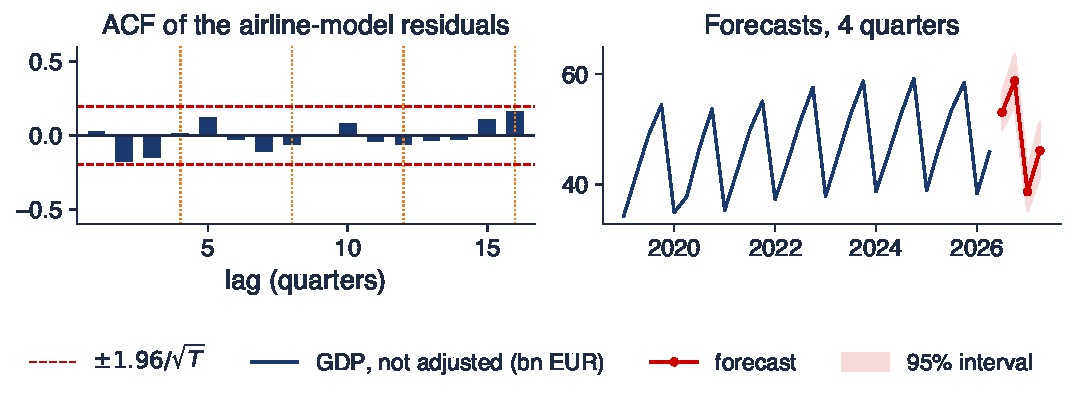
\includegraphics[width=0.96\textwidth,height=0.33\textheight,keepaspectratio]{ch4_sem_b1.pdf}
\end{center}
\vspace{-2mm}
\begin{itemize}
    \item $\hat\theta = -0{,}171$ (0{,}109): nesemnificativ; $\hat\Theta = -0{,}585$ (0{,}072); $\hat\sigma = 3{,}05\%$; $Q^*(8) = 9{,}30$, p = 0{,}157: fără autocorelație în reziduuri
    \item Prognozele din T3 2026: 53{,}1; 58{,}7; 38{,}7; 46{,}1 mld. EUR; primul interval $[50{,}0; 56{,}4]$, al patrulea $[41{,}5; 51{,}2]$
    \item Creșterea anuală implicată: $-$0{,}84\%; 0{,}52\%; 0{,}83\%; 0{,}53\%
    \item Interpretare: prognoza sezonieră este o medie ponderată exponențial a tiparelor sezoniere trecute, cu ponderea $1 + \hat\Theta = 0{,}42$ pentru anul cel mai recent; $\Theta = -1$ ar însemna un tipar fix, $\Theta = 0$ un tipar care se schimbă liber: tiparul PIB-ului evoluează lent
\end{itemize}\quantlet{TSA\_ch4\_seminar}{\qlurl{TSA_ch4_seminar}}
\end{frame}

\begin{frame}{B2: producția industrială și zilele lucrătoare [Propus]}
\itemsize{\footnotesize}
\begin{itemize}
\item \textbf{Întrebarea}: explică numărul zilelor lucrătoare o parte din mișcările lunare ale producției industriale din România?
\item \textbf{Date}: Eurostat, producția industrială neajustată, 2010--iulie 2026, $y_t = 100\ln Y_t$; variabile dummy pentru aprilie și mai 2020; model: B1
\item \textbf{Cerințe}
\begin{enumerate}
    \item Estimați modelul airline cu și fără numărul zilelor lucrătoare ca regresor și comparați AICc și $Q^*(24)$.
    \item Adăugați două alternative cu zile lucrătoare, $(2,1,0)(0,1,1)_{12}$ și $(1,1,1)(0,1,1)_{12}$, și alegeți un model.
    \item Raportați coeficientul zilelor lucrătoare cu eroarea lui standard și prognozați următoarele 12 luni.
    \item Interpretare: de ce trebuie eliminat efectul zilelor lucrătoare înainte de a compara două luni?
\end{enumerate}
\item \textbf{Raportați}: un tabel cu AICc și valori p, un coeficient, graficul prognozei și o frază
\item Notebook: secțiunea B2
\end{itemize}
\end{frame}

\ifsolutions
\begin{frame}{B2: rezolvare [Propus]}
\itemsize{\scriptsize}
\begin{center}
\includegraphics[width=0.96\textwidth,height=0.30\textheight,keepaspectratio]{ch4_sem_b2.pdf}
\end{center}
\vspace{-2mm}
\begin{center}
\scriptsize
\begin{tabular}{lrr}
\toprule
Modelul & AICc & $Q^*(24)$, p \\
\midrule
$(0,1,1)(0,1,1)_{12}$ & 1023{,}8 & $<$\,0{,}001 \\
$(0,1,1)(0,1,1)_{12}$ + WD & \textbf{888{,}0} & 0{,}798 \\
$(2,1,0)(0,1,1)_{12}$ & 1012{,}0 & 0{,}003 \\
$(2,1,0)(0,1,1)_{12}$ + WD & 889{,}6 & 0{,}757 \\
$(1,1,1)(0,1,1)_{12}$ + WD & 890{,}1 & 0{,}742 \\
\bottomrule
\end{tabular}
\end{center}
\begin{itemize}
    \item Cel mai bun: airline + zile lucrătoare (WD); o zi lucrătoare în plus crește producția cu 2{,}49\% (eroarea standard 0{,}15); $\hat\theta = -0{,}481$, $\hat\Theta = -0{,}771$; fără WD reziduurile nu trec testul Ljung--Box, iar $\hat\Theta$ ajunge la $-$0{,}998
    \item Interpretare: o lună cu două zile lucrătoare în plus are o producție cu aproximativ 5{,}0\% mai mare doar din motive de calendar; comparația fără această corecție confundă calendarul cu ciclul economic
\end{itemize}
\end{frame}
\fi

\begin{frame}{B3: validare încrucișată pentru consumul zilnic de electricitate [Rezolvat]}
\itemsize{\footnotesize}
\begin{itemize}
\item \textbf{Întrebarea}: prognozează o regresie cu termeni Fourier și variabile dummy pentru sărbători consumul zilnic mai bine decît SARIMA și metoda sezonieră naivă?
\item \textbf{Date}: ENTSO-E, consumul mediu zilnic în România (GW), 2022--2026; 13 origini la 28 de zile, de la 30 iunie 2025 la 1 iunie 2026, orizont de 14 zile
\item \textbf{Cerințe}
\begin{enumerate}
    \item La fiecare origine, estimați metoda sezonieră naivă (perioada 7), SARIMA$(1,0,1)(0,1,1)_7$ și o DHR (4 perechi Fourier anuale, variabile dummy pentru zilele săptămînii și sărbători, erori ARMA(1,1)).
    \item Calculați MAE și MASE pentru fiecare metodă, pe toate originile și orizonturile.
    \item Testați DHR față de SARIMA cu testul DM pe media erorilor pătratice din fiecare fereastră (o valoare pe origine), cu corecția HLN.
    \item Comparați MAE în zilele de sărbătoare legală cu MAE în zilele obișnuite.
    \item Interpretare: de ce este cîștigul DHR cel mai mare în zilele de sărbătoare legală?
\end{enumerate}
\item \textbf{Raportați}: un tabel cu MAE și MASE, un test, graficul și o frază
\item Notebook: secțiunea B3
\end{itemize}
\end{frame}

\begin{frame}{B3: rezolvare [Rezolvat]}
\itemsize{\scriptsize}
\begin{center}
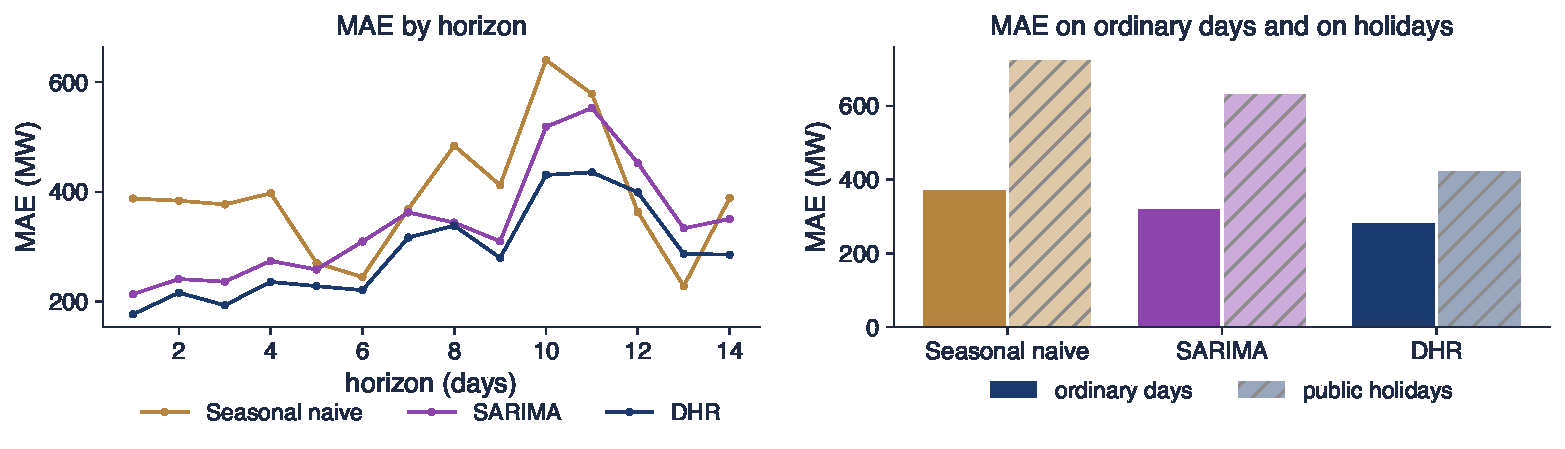
\includegraphics[width=0.96\textwidth,height=0.32\textheight,keepaspectratio]{ch4_sem_b3.pdf}
\end{center}
\vspace{-2mm}
\begin{center}
\scriptsize
\begin{tabular}{lrrrr}
\toprule
Metoda & MAE (MW) & MASE & sărbători & alte zile \\
\midrule
Sezonieră naivă & 395 & 1{,}28 & 723 & 372 \\
SARIMA & 340 & 1{,}10 & 630 & 319 \\
DHR & \textbf{289} & \textbf{0{,}94} & 422 & 280 \\
\bottomrule
\end{tabular}
\end{center}
\begin{itemize}
    \item Scala MASE: MAE în eșantion a metodei sezoniere naive săptămînale, 309 MW; DM (HLN), DHR față de SARIMA: $-$1{,}96, p = 0{,}073; față de metoda sezonieră naivă: $-$2{,}73, p = 0{,}018
    \item Interpretare: SARIMA și metoda sezonieră naivă cunosc doar „acum o săptămînă”; o sărbătoare care cade într-o zi lucrătoare arată pentru ele ca o zi obișnuită, în timp ce DHR are variabile dummy care scad 0{,}37 GW într-o zi de sărbătoare legală și 0{,}56 GW în zilele de Paște
\end{itemize}\quantlet{TSA\_ch4\_seminar}{\qlurl{TSA_ch4_seminar}}
\end{frame}

\begin{frame}{B4: sezonalitatea inflației lunare [Propus]}
\itemsize{\footnotesize}
\begin{itemize}
\item \textbf{Întrebarea}: este tiparul sezonier al inflației lunare din România suficient de puternic pentru a îmbunătăți prognozele pe o lună?
\item \textbf{Date}: IAPC, România, 2010--2026; $\pi_t = 100\,\Delta\ln P_t$ (\% pe lună); model: B3
\item \textbf{Cerințe}
\begin{enumerate}
    \item Regresați $\pi_t$ (2010--2019) pe 12 variabile dummy lunare și testați egalitatea mediilor lunare cu un test $F$.
    \item Estimați modelul airline pentru $100\ln P_t$ și raportați $\hat\theta$ și $\hat\Theta$.
    \item Din origini lunare începînd cu ianuarie 2016, prognozați $\pi$ din luna următoare cu SARIMA, metoda sezonieră naivă și media ultimelor 12 luni; comparați MAE.
    \item Testați SARIMA față de ambele repere cu testul DM (erori pătratice).
    \item Interpretare: este tiparul sezonier suficient de puternic pentru a îmbunătăți prognozele pe o lună?
\end{enumerate}
\item \textbf{Raportați}: un test $F$, două estimări, trei valori MAE, două teste DM și o frază
\item Notebook: secțiunea B4
\end{itemize}
\end{frame}

\ifsolutions
\begin{frame}{B4: rezolvare [Propus]}
\itemsize{\scriptsize}
\begin{center}
\includegraphics[width=0.96\textwidth,height=0.30\textheight,keepaspectratio]{ch4_sem_b4.pdf}
\end{center}
\vspace{-2mm}
\begin{itemize}
    \item $F = 2{,}71$, p = 0{,}004: mediile lunare diferă; ianuarie 0{,}45\%, iunie $-$0{,}37\% (alimente proaspete), august $-$0{,}10\%, octombrie 0{,}49\%
    \item Airline: $\hat\theta = 0{,}356$ (0{,}060), $\hat\Theta = -0{,}782$ (0{,}063); 127 de prognoze, februarie 2016--august 2026: MAE SARIMA 0{,}312, sezonieră naivă 0{,}427, media pe 12 luni 0{,}313
    \item DM (HLN): SARIMA față de metoda sezonieră naivă $-$3{,}27 (p = 0{,}001); față de media pe 12 luni 0{,}08 (p = 0{,}935)
    \item Interpretare: tiparul sezonier există, dar este mic în raport cu zgomotul lunar; SARIMA bate copierea lunii de anul trecut, dar nu bate media simplă pe 12 luni
\end{itemize}
\end{frame}
\fi


%=============================================================================
\section{Partea C: întrebări deschise și critica unui răspuns AI}
%=============================================================================

\begin{frame}{C1: turismul după pandemie [Propus]}
\itemsize{\footnotesize}
\begin{itemize}
\item \textbf{Întrebarea}: ce eșantion de antrenare dă prognoze mai bune ale înnoptărilor turistice pentru 2023--2025: datele pînă în 2019 sau datele pînă în 2022?
\item \textbf{Date}: Eurostat, înnoptări în unitățile de cazare turistică, România, lunar, 2005--2025; model: B1
\item \textbf{Cerințe}
\begin{enumerate}
    \item Estimați modelul airline pentru $\ln y_t$ pînă în decembrie 2019 și prognozați 2023--2025.
    \item Repetați cu datele pînă în decembrie 2022.
    \item Comparați ambele cu prognoza sezonieră naivă care repetă anul 2022, folosind MAPE (eroarea procentuală absolută medie).
    \item Propuneți un tratament mai bun pentru 2020--2021 (variabile dummy de intervenție, un eșantion mai scurt, TBATS sau Prophet) și schițați-l ca proiect de echipă.
\end{enumerate}
\item \textbf{Raportați}: trei valori MAPE, graficul și un plan de proiect
\item Notebook: secțiunea C1
\end{itemize}
\end{frame}

\ifsolutions
\begin{frame}{C1: analiză de referință [Propus]}
\itemsize{\scriptsize}
\begin{center}
\includegraphics[width=0.96\textwidth,height=0.36\textheight,keepaspectratio]{ch4_sem_c1.pdf}
\end{center}
\vspace{-2mm}
\begin{itemize}
    \item MAPE 2023--2025: airline estimat pînă în 2019 20{,}0\%; estimat pînă în 2022 37{,}7\%; sezonieră naivă (2022 repetat) 11{,}6\%; înnoptări: 29{,}9 milioane în 2019, 29{,}7 milioane în 2025
    \item Interpretare: prăbușirea din 2020 intră în datele diferențiate ca șocuri foarte mari, iar modelul estimat pînă în 2022 extrapolează revenirea; modelul vechi ignoră ruptura; cea mai simplă prognoză cîștigă. Un proiect: analiza intervenției cu variabile dummy pentru 2020--2021, comparată cu origini mobile
\end{itemize}
\end{frame}
\fi

\begin{frame}{C2: verificați un răspuns AI [Propus]}
\itemsize{\scriptsize}
\begin{itemize}
    \item Un student a cerut unui asistent AI informații despre modelele sezoniere. Răspunsul:
    \item \aiprompt{(a) SARIMA(0,1,1)(0,1,1)4 are patru parametri MA, la decalajele 1, 4 și 5, plus varianța zgomotului.}
    \item \aiprompt{(b) Dacă ACF a seriei lunare diferențiate are o singură valoare semnificativă la decalajul 12, iar PACF descrește la 12, 24, 36, folosiți un AR(1) sezonier.}
    \item \aiprompt{(c) PIB-ul neajustat al României a scăzut cu aproximativ 34\% în primul trimestru din 2026 față de al patrulea trimestru din 2025: o recesiune profundă.}
    \item \aiprompt{(d) DM = $-$2,3 cu d = L(e1) - L(e2) arată că prognoza 2 este semnificativ mai precisă.}
    \item \aiprompt{(e) TBATS cu perioadele 7 și 365,25 surprinde scăderea consumului de electricitate de Paște.}
    \item \aiprompt{(f) Media cu ponderi egale a două prognoze nedeplasate nu are niciodată un MSE mai mare decît media celor două MSE.}
    \item Cerințe
    \begin{itemize}
        \item 1. Pentru fiecare afirmație, precizați dacă este corectă; dacă nu, dați afirmația corectă și, unde se poate, valoarea corectă din notebook (secțiunea C2).
        \item 2. Raportați: o listă de șase verdicte, fiecare cu un rînd de justificare.
    \end{itemize}
\end{itemize}
\end{frame}

\ifsolutions
\begin{frame}{C2: rezolvare [Propus]}
\itemsize{\scriptsize}
\begin{itemize}
    \item (a) Greșit: doi parametri MA, $\theta$ și $\Theta$; coeficientul de la decalajul 5 este produsul $\theta\Theta$ (A2, A3)
    \item (b) Greșit: o ACF care se anulează după decalajul 12, cu PACF sezonieră descrescătoare, indică un MA(1) sezonier (A4)
    \item (c) Greșit: scăderea este sezonieră (T1 este mereu cel mai slab trimestru): neajustat $-$34{,}3\%, ajustat (SCA) $-$0{,}06\% în T1 2026
    \item (d) Greșit: $\bar d < 0$ favorizează prognoza 1; semnificația cere și ca $|\mathrm{HLN}|$ să depășească valoarea critică $t(n - 1)$ (A5)
    \item (e) Greșit: Paștele ortodox se mută între aprilie și mai; o perioadă fixă nu îl poate urmări; este nevoie de un regresor de sărbătoare, ca în DHR din B3
    \item (f) Corect: $\mathrm{MSE}(0{,}5) = (\sigma_1^2 + \sigma_2^2 + 2\rho\sigma_1\sigma_2)/4 \le (\sigma_1^2 + \sigma_2^2)/2$, deoarece $2\rho\sigma_1\sigma_2 \le \sigma_1^2 + \sigma_2^2$ (A6)
\end{itemize}\quantlet{TSA\_ch4\_seminar}{\qlurl{TSA_ch4_seminar}}
\end{frame}
\fi


%=============================================================================
\section{Încheiere}
%=============================================================================

\begin{frame}{Idei de reținut}
\itemsize{\small}
\begin{itemize}
    \item $\Delta_s$ elimină un tipar sezonier stabil; $\Delta\Delta_s$ elimină și trendul; prognoza sezonieră naivă este reperul
    \item SARIMA înmulțește un polinom obișnuit și unul sezonier: modelul airline are doi parametri și valori nenule ale ACF la $1$, $s - 1$, $s$, $s + 1$
    \item Efectele de calendar (zile lucrătoare, Paște, sărbători legale) sînt cunoscute dinainte: introduceți-le ca regresori
    \item Comparați prognozele în afara eșantionului, cu origini mobile, MASE și testul DM; un cîștig vizibil nu este întotdeauna unul semnificativ
    \item Combinarea prognozelor este o asigurare ieftină: rareori este cea mai slabă și deseori este aproape de cea mai bună
\end{itemize}
\end{frame}

\begin{frame}{După seminar}
\itemsize{\small}
\begin{itemize}
    \item Cursul 4 deduce formulele de azi și adaugă rădăcinile unitare sezoniere, ajustarea sezonieră (X-13ARIMA-SEATS), sezonalitatea multiplă, TBATS și Prophet
    \item Încercați cerințele [Propus] în notebook; TBATS și Prophet se instalează opțional acolo
    \item C1 poate deveni un proiect de echipă: prognoza turismului sau a consumului de electricitate din România, cu o comparație pe origini mobile a mai multor modele
    \item Lectură: \refHP, cap.~4--5; \refFPPsar; \refFPPcv; \refDM
    \item \textbf{Seminarul are rol de exercițiu și nu se notează; rezolvările cerințelor [Propus] se discută la seminar}
\end{itemize}
\end{frame}


%=============================================================================
\section{Bibliografie}
%=============================================================================

\begin{frame}{Bibliografie}
\itemsize{\tiny}
\begin{itemize}
    \item Bates, J. M., \& Granger, C. W. J. (1969). The combination of forecasts. \textit{Journal of the Operational Research Society}, 20(4), 451--468. \href{https://doi.org/10.1057/jors.1969.103}{doi:10.1057/jors.1969.103}
    \item Box, G. E. P., Jenkins, G. M., \& Reinsel, G. C. (2008). \textit{Time Series Analysis: Forecasting and Control} (4th ed.). Wiley. \href{https://doi.org/10.1002/9781118619193}{doi:10.1002/9781118619193}
    \item Diebold, F. X., \& Mariano, R. S. (1995). Comparing predictive accuracy. \textit{Journal of Business \& Economic Statistics}, 13(3), 253--263. \href{https://doi.org/10.1080/07350015.1995.10524599}{doi:10.1080/07350015.1995.10524599}
    \item Harvey, D., Leybourne, S., \& Newbold, P. (1997). Testing the equality of prediction mean squared errors. \textit{International Journal of Forecasting}, 13(2), 281--291. \href{https://doi.org/10.1016/S0169-2070(96)00719-4}{doi:10.1016/S0169-2070(96)00719-4}
    \item Huang, C., \& Petukhina, A. (2022). \textit{Applied Time Series Analysis and Forecasting with Python}. Springer. \href{https://doi.org/10.1007/978-3-031-13584-2}{doi:10.1007/978-3-031-13584-2}
    \item Hyndman, R. J., \& Athanasopoulos, G. (2021). \textit{Forecasting: Principles and Practice} (3rd ed.). OTexts. \href{https://otexts.com/fpp3/}{otexts.com/fpp3}
    \item Hyndman, R. J., \& Koehler, A. B. (2006). Another look at measures of forecast accuracy. \textit{International Journal of Forecasting}, 22(4), 679--688. \href{https://doi.org/10.1016/j.ijforecast.2006.03.001}{doi:10.1016/j.ijforecast.2006.03.001}
    \item Ljung, G. M., \& Box, G. E. P. (1978). On a measure of lack of fit in time series models. \textit{Biometrika}, 65(2), 297--303. \href{https://doi.org/10.1093/biomet/65.2.297}{doi:10.1093/biomet/65.2.297}
    \item Tashman, L. J. (2000). Out-of-sample tests of forecasting accuracy: an analysis and review. \textit{International Journal of Forecasting}, 16(4), 437--450. \href{https://doi.org/10.1016/S0169-2070(00)00065-0}{doi:10.1016/S0169-2070(00)00065-0}
\end{itemize}
\end{frame}

\end{document}
